\documentclass[a4paper, 11pt]{article}

\usepackage[DD2380, handin]{blackboard}
\classno{}

\title{A3.PP}
\renewcommand{\and}{\wedge}
\usepackage{float}

\begin{document}
	\section{Beekeeper}
	See the zipped files. \\[6pt]
    I believe I have programmed correctly, however the provided online solver, and PDDL4 do not solve the problem with a minimal total cost, so I was not able to verify that the written code was indeed correct. 
    
    
	\section{Einstein puzzle with a twist}
	\subsection{Constructing sentences}
	\begin{alignedequations}{3}
		\text{S1}\quad & House(Bob) = Red \\
		\text{S2}\quad & Drink(Alice) = Snaps \\
		\text{S3}\quad & Fear(Ted) = Elevators \\
		\text{S4}\quad & Roommate(Carol, Ted) \\
		\text{S5}\quad & \forall x ~  Fear(x) = Elevators \Rightarrow House(x) = Blue \\
		\text{S6}\quad & \forall x ~ House(x) = Red \Rightarrow Fear(x) = Spiders \\
		\text{S7}\quad & \forall x ~  Drink(x) = Snaps \Rightarrow House(x) = Red \\
		\text{S8}\quad & \forall x ~  Neighbor(Bob, x) \Rightarrow Drink(x) = Beer \\
		\text{S9}\quad & \forall x,y ~ Roommate(x, y) \and Fear(y) = Elevators \Rightarrow Fear(x) = Spiders \\
		\text{S10}\quad & \forall x,y ~  Neighbor(x, y) \and Drink(x) = Milk \Rightarrow Music(y) = Beatles \\
		\text{S11}\quad & \forall x ~ Roomate(Alice, x) \and Fear(x) = Spider \Rightarrow Drink(x) = Milk \\
		\text{S12}\quad & \forall x,y ~ Roommate(x, y) \and Drink(x) = Snaps \Rightarrow Music(y) = Beatles \\
		\text{S13}\quad & \forall x ~ Neighbor(Ted, x) \and Drink(x) = Snaps \and Fear(x) = Spiders \Rightarrow Music(x) = ABBA \\
	\end{alignedequations}
	
	\subsection{Inference using generalized modus ponens}
	Letting $S3, ~S4$ be $p^\prime_1, ~p^\prime_2$ and splitting $S9$ into $p_1 = Roommate(x, y) \and Fear(y) = Elevators$ and $q = Fear(x) = Spiders$ we get
	
	\begin{equation} \footnotesize
		\frac{Fear(Ted) = Elevators, ~Roommate(Carol, Ted) \quad (Roommate(x, y) \and Fear(y) = Elevators \Rightarrow Fear(x) = Spiders)}{Fear(Carol) = Spiders}
	\end{equation} 
	where $\theta = \{y/Ted, ~ x/Carol\}$
	
	\subsection{Introducing CNF}
	\begin{alignedequations}{2}
		\text{C1}\quad & House(Bob) = Red \\
		\text{C2}\quad & Drink(Alice) = Snaps \\
		\text{C3}\quad & Fear(Ted) = Elevators \\
		\text{C4}\quad & Roommates(Carol, Ted) \\
		\text{C5}\quad & \neg Fear(x) = Elevators \vee House(x) = Blue \\
		\text{C6}\quad & \neg House(x) = Red \vee Fear(x) = Spiders \\
		\text{C7}\quad & \neg Drink(x) = Snaps \vee House(x) = Red \\
		\text{C8}\quad & \neg Neighbor(Bob, x) \vee Drink(x) = Beer \\
		\text{C9}\quad & \neg Roommates(x, y) \vee \neg Fear(y) = Elevators \vee Fear(x) = Spiders \\
		\text{C10}\quad & \neg Neighbors(x, y) \vee \neg Drink(x) = Milk \vee Music(y) = Beatles \\
		\text{C11}\quad & \neg Roommates(Alice, x) \vee \neg Fear(x) = Spider \vee Drink(x) = Milk \\
		\text{C12}\quad & \neg Roommates(x, y) \vee \neg Drink(x) = Snaps \vee Music(y) = Beatles \\
		\text{C13}\quad & \neg Neighbors(Ted, x) \vee \neg Drink(x) = Snaps \vee \neg Fear(x) = Spiders \vee Music(x) = ABBA \\
	\end{alignedequations} \\

    Following the $HaveCake/BakedCake$ example in the lecture slides.
	
	\subsection{Inference of music}

	\begin{alignedequations}{2}
		\text{C14}\quad & \neg Roommates(x,y) \vee \neg House(x) = z \vee House(y) = z \\
		& \text{If two persons are roomates, they live in the same house. } \\[-4pt]
		& \text{(Or more specifially if one lives in a house, the other live in the same house)} \\
		\text{C15}\quad & \neg House(x) = z \vee \neg House(y) = z \vee Roommates(x, y)  \\ 
		& \text{If two persons live in the same house, they are roommates.} \\
		\text{C16}\quad & \neg Roommates(x,y) \vee Roomates(y,x) \\
		& \text{Roommates are mutually each others roommates. } \\
		\text{C17}\quad & \neg House(x) = Red \vee \neg House(y) = Blue \vee Neighbors(x,y) \\
		& \text{If two persons live in different houses (Red and Blue), they are neighbors.} \\
		\text{C18}\quad & \neg Neighbors(x,y) \vee Neighbors(y,x) \\
		& \text{Neighbors are mutually each others neighbors. } \\
	\end{alignedequations}

    \subsubsection{Inference with the resolution rule}

	\begin{alignedequations}{2}
		&\frac{\text{C2: } Drink(Alice) = Snaps, \quad \text{C7: } \neg Drink(x) = Snaps \vee House(x) = Red}{\text{C19: } House(Alice) = Red}, \quad \theta = \{x / Alice\}
	\end{alignedequations}	
	
	\begin{alignedequations}{2}
		&\frac{
			\text{C19: } House(Alice) = Red, \quad \text{C15: } \neg House(x) = z \vee \neg House(y) = z \vee Roommates(x, y) 
		}{
			\text{C20: } \neg House(y) = Red \vee Roommates(Alice, y)
		}, \quad \theta = \{x / Alice, z / Red\}
	\end{alignedequations}	
	
	\begin{alignedequations}{2}
		&\frac{
			\text{C1: } House(Bob) = Red, \quad \text{C20: } \neg House(y) = Red \vee Roommates(Alice, y)
		}{
			\text{C21: } Roommates(Alice, Bob)
		}, \quad \theta = \{y / Bob\}
	\end{alignedequations}	
	
	\begin{alignedequations}{2}
		& \frac{
		\text{C21: } Roommates(Alice, Bob), \quad \text{C12: } \neg Roommates(x, y) \vee \neg Drink(x) = Snaps \vee Music(y) = Beatles
		}{
			\text{C22: } \neg Drink(Alice) = Snaps \vee Music(Bob) = Beatles
		}, \\
	 & \quad \theta = \{x / Alice, y / Bob\}
	\end{alignedequations}	
	
	\begin{alignedequations}{2}
		&\frac{
			\text{C2: } Drink(Alice) = Snaps, \quad \text{C22: } \neg Drink(Alice) = Snaps \vee Music(Bob) = Beatles
		}{
			\text{C23: } Music(Bob) = Beatles
		}, \quad \theta = \emptyset
	\end{alignedequations}	
	
	Therefore Bob likes the Beatles. Furthermore \\
	
	\begin{alignedequations}{2}
	&\frac{
		\text{C19: } House(Alice) = Red, \quad \text{C17: } \neg House(x) = Red \vee \neg House(y) = Blue \vee Neighbors(x,y)
	}{
		\text{C24: } \neg House(y) = Blue \vee Neighbors(Alice, y)
	}, \quad \theta = \{x / Alice\}
	\end{alignedequations}	
	
	\begin{alignedequations}{2}
		&\footnotesize\frac{
			\text{C4: } Roommates(Carol, Ted), \quad \text{C9: } \neg Roommates(x, y) \vee \neg Fear(y) = Elevators \vee Fear(x) = Spiders
		}{
			\text{C25: } \neg Fear(Ted) = Elevators \vee Fear(Carol) = Spiders
		}, \\
		&\quad \theta = \{x / Carol, y / Ted\}
	\end{alignedequations}

	\begin{alignedequations}{2}
		&\footnotesize\frac{
			\text{C3: } Fear(Ted) = Elevators, \quad \text{C25: } \neg Fear(Ted) = Elevators \vee Fear(Carol) = Spiders
		}{
			\text{C26: } Fear(Carol) = Spiders
		}, \quad \theta = \emptyset
	\end{alignedequations}	

	\begin{alignedequations}{2}
		&\frac{
			\text{C26: } Fear(Ted) = Elevators, \quad \text{C5: } \neg Fear(x) = Elevators \vee House(x) = Blue
		}{
			\text{C27: } House(Ted) = Blue
		}, \quad \theta = \{x / Ted\}
	\end{alignedequations}	

	\begin{alignedequations}{2}
		&\frac{
			\text{C4: } Roommates(Carol, Ted), \quad \text{C16: } \neg Roommates(x,y) \vee Roomates(y,x)
		}{
			\text{C28: } Roommates(Ted,Carol)
		}, &\quad \theta = \{x / Carol, y / Ted\}
\end{alignedequations}	
	
	\begin{alignedequations}{2}
		&\frac{
			\text{C28: } Roommates(Ted,Carol), \quad \text{C14: } Roommates(x,y) \vee \neg House(x) = z \vee House(y) = z
		}{
			\text{C29: } \neg House(Ted) = z \vee House(Carol) = z
		}, \\
		&\quad \theta = \{x / Ted, y / Carol\}
	\end{alignedequations}	

	\begin{alignedequations}{2}
		&\frac{
			\text{C27: } House(Ted) = Blue, \quad \text{C29: } \neg House(Ted) = z \vee House(Carol) = z
		}{
			\text{C30: } House(Carol) = Blue
		}, \quad \theta = \{z / Blue\}
	\end{alignedequations}

	\begin{alignedequations}{2}
		&\frac{
			\text{C30: } House(Ted) = Blue, \quad \text{C24: } \neg House(y) = Blue \vee Neighbors(Alice, y)
		}{
			\text{C31: } Neighbors(Alice,Ted)
		}, \quad \theta = \{y / Ted\}
	\end{alignedequations}	

	\begin{alignedequations}{2}
		&\frac{
			\text{C19: } House(Alice) = Red, \quad \text{C9: } \neg House(x) = Red \vee Fear(x) = Spiders
		}{
			\text{C32: } Fear(Alice) = Spiders
		}, \quad \theta = \{x / Alice\}
	\end{alignedequations}	

	\begin{alignedequations}{2}
    &\frac{
        \text{C31: } Neighbors(Alice,Ted), \quad \text{C18: }\neg Neighbors(x, y) \vee Neighbors(y,x)
    }{
        \text{C33: } Neighbors(Ted,Alice)
    }, \quad \theta = \{x / Alice, y / Ted\}
\end{alignedequations}	


	\begin{alignedequations}{2}
		&\tfrac{
			\text{C31: } Neighbors(Alice,Ted), \quad \text{C33: }\neg Neighbor(Ted, x) \vee \neg Drink(x) = Snaps \vee \neg Fear(x) = Spiders \vee Music(x) = ABBA
		}{
			\text{C34: } \vee \neg Drink(Alice) = Snaps \vee \neg Fear(Alice) = Spiders \vee Music(Alice) = ABBA
		}, \\
	&\footnotesize\quad \theta = \{x / Alice\}
	\end{alignedequations}	

	\begin{alignedequations}{2}
		&\tfrac{
			\text{C2: } Drink(Alice) = Snaps, \quad \text{C34: } \vee \neg Drink(Alice) = Snaps \vee \neg Fear(Alice) = Spiders \vee Music(Alice) = ABBA
		}{
			\text{C35: } \neg Fear(Alice) = Spiders \vee Music(Alice) = ABBA
		}, \\
		&\footnotesize\quad \theta = \emptyset
	\end{alignedequations}	

	\begin{alignedequations}{2}
		&\frac{
			\text{C32: } Fear(Alice) = Spiders, \quad \text{C35: } \neg Fear(Alice) = Spiders \vee Music(Alice) = ABBA
		}{
			\text{C36: } Music(Alice) = ABBA
		}, \\
		&\footnotesize\quad \theta = \emptyset
	\end{alignedequations}	
	
	So Alice likes ABBA. Additionally: \\
	
	\begin{alignedequations}{2}
		&\frac{
			\text{C1: } House(Bob) = Red, \quad \text{C6: } \neg House(x) = Red \vee Fear(x) = Spiders
		}{
			\text{C37: } Fear(Bob) = Spiders
		}, &\footnotesize\quad \theta = \{x / Bob\}
	\end{alignedequations}

	\begin{alignedequations}{2}
		&\frac{
			\text{C1: } House(Bob) = Red \quad \text{C17: } \neg House(x) = Red \vee \neg House(y) = Blue \vee Neighbors(x,y) 
		}{
			\text{C38: } \neg House(y) = Blue \vee Neighbors(Bob,y) 
		}, \quad \theta = \{x / Bob\}
	\end{alignedequations}

	\begin{alignedequations}{2}
		&\frac{
		\text{C29: } House(Ted) = Blue, \quad \text{C38: } \neg House(y) = Blue \vee Neighbors(Bob,y) 
		}{
			\text{C39: } Neighbors(Bob,Ted)
		}, \quad \theta = \{ y / Ted\}
	\end{alignedequations}
	
	\begin{alignedequations}{2}
		&\frac{
			\text{C21: } Roomates(Alice,Bob), \quad \text{C11: } \neg Roommates(Alice, x) \vee \neg Fear(x) = Spider \vee Drink(x) = Milk 
		}{
			\text{C40: } \neg Fear(Bob) = Spider \vee Drink(Bob) = Milk 
		}, \\
		&\footnotesize\quad \theta = \{x / Bob\}
	\end{alignedequations}

	\begin{alignedequations}{2}
		&\frac{
			\text{C37: } Fear(Bob) = Spiders, \quad \text{C38: } \neg Fear(Bob) = Spider \vee Drink(Bob) = Milk 
		}{
			\text{C41: } Drink(Bob) = Milk
		}, \quad \theta = \{x / Bob\}
	\end{alignedequations}
	
	\begin{alignedequations}{2}
		&\frac{
			\text{C39: } Neighbors(Bob,Ted), \quad \text{C10: } \neg Neighbors(x, y) \vee \neg Drink(x) = Milk \vee Music(y) = Beatles 
		}{
			\text{C42: } \neg Drink(Bob) = Milk \vee Music(Ted) = Beatles 
		}, \\
		&\footnotesize\quad \theta = \{x / Bob, y / Ted\}
	\end{alignedequations}

	\begin{alignedequations}{2}
		&\frac{
			\text{C41: } Drink(Bob) = Milk, \quad \text{C42: } \neg Drink(Bob) = Milk \vee Music(Ted) = Beatles 
		}{
			\text{C43: } Music(Ted) = Beatles
		}, \quad \theta = \emptyset
	\end{alignedequations}

	So Ted listens to the Beatles. Lastly: \\
	
	\begin{alignedequations}{2}
		&\frac{
			\text{C1: } House(Bob) = Red, \quad \text{C17: } \neg House(x) = Red \vee \neg House(y) = Blue \vee Neighbors(x,y) 
		}{
			\text{C44: } \neg House(Carol) = Blue \vee Neighbors(Bob,Carol)
		}, \\
	& \quad \theta = \{x / Bob, y / Carol\}
	\end{alignedequations} 

	\begin{alignedequations}{2}
		&\frac{
			\text{C26: } House(Carol) = Blue, \quad \text{C44: } \neg House(Carol) = Blue \vee Neighbors(Bob,Carol)
		}{
			\text{C45: } Neighbors(Bob,Carol)
		}, \\
	& \quad \theta = \{x / Bob, y / Carol\}
	\end{alignedequations} 

	\begin{alignedequations}{2}
		&\frac{
			\text{C45: } Neighbors(Bob,Carol), \quad \text{C10: } \neg Neighbors(x, y) \vee \neg Drink(x) = Milk \vee Music(y) = Beatles 
		}{
			\text{C46: } \neg Drink(Bob) = Milk \vee Music(Carol) = Beatles 
		}, \\
		&\footnotesize\quad \theta = \{x / Bob, y / Carol\}
	\end{alignedequations}

	\begin{alignedequations}{2}
		&\frac{
			\text{C38: } Drink(Bob) = Milk, \quad \text{C46: } \vee \neg Drink(x) = Milk \vee Music(y) = Beatles 
		}{
			\text{C47: } Music(Carol) = Beatles
		}, \quad \theta = \emptyset
	\end{alignedequations}

	So Carol is also a fan of the Beatles. \\
	Summed up: 
	\begin{equation*}
		\begin{cases}
			Music(Ted) = Beatles \\
			Music(Carol) = Beatles \\
			Music(Bob) = Beatles \\
			Music(Alice) = ABBA
		\end{cases}
	\end{equation*}
    
    {\tiny Some resolutions above may have been unnecessary. }
	
	\subsection{Resolving two clauses in two different ways}
	\begin{equation}
		\frac{House(Ted) = Red \vee Fear(Alice) = Spiders, \quad \neg House(x) = Red \vee \neg Fear(x) = Spiders}{???}
	\end{equation}
	Can be resolved in two different ways:
	\begin{equation}
		\frac{House(Ted) = Red \vee Fear(Alice) = Spiders, \quad \neg House(x) = Red \vee \neg Fear(x) = Spiders}{\neg Fear(Ted) = Spiders}, ~ \theta = \{x/Ted\}
	\end{equation}
	or 
	\begin{equation}
		\frac{House(Ted) = Red \vee Fear(Alice) = Spiders, \quad \neg House(x) = Red \vee \neg Fear(x) = Spiders}{\neg House(Alice) = Red}, ~ \theta = \{x/Alice\}
	\end{equation}
    with toally different meanings.
	\section{Treasure hunt}
	\subsection{State space}
	
	\subsubsection{Graph}
	
	\tikzset{every picture/.style={line width=0.75pt}} %set default line width to 0.75pt        
	\begin{figure}[h]\centering
	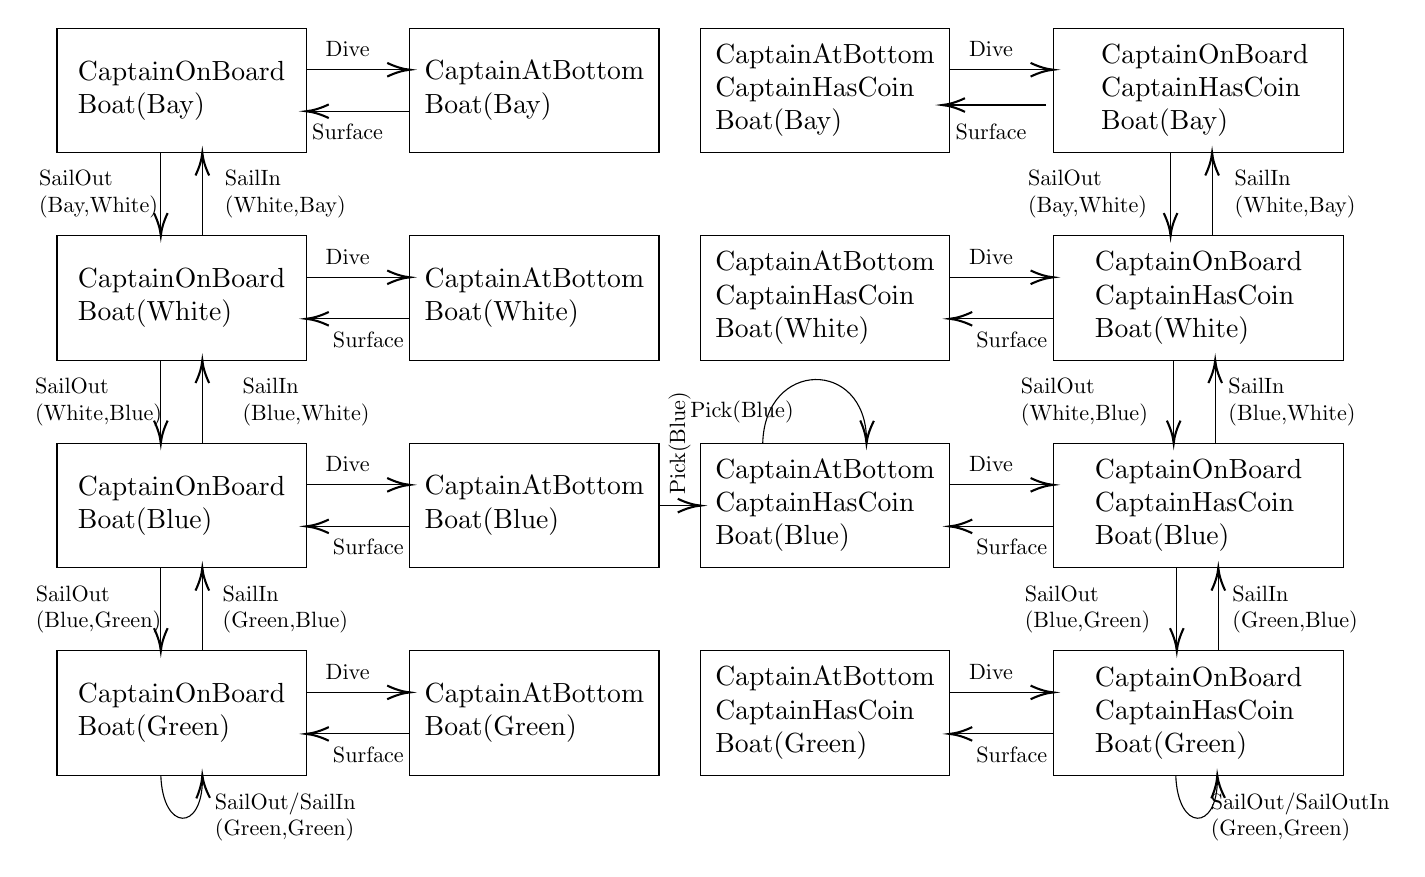
\begin{tikzpicture}[x=0.75pt,y=0.75pt,yscale=-1,xscale=1]
	%uncomment if require: \path (0,480); %set diagram left start at 0, and has height of 480
	
	%Shape: Rectangle [id:dp689946327869519] 
	\draw   (20,20) -- (140,20) -- (140,80) -- (20,80) -- cycle ;
	%Shape: Rectangle [id:dp698201888405773] 
	\draw   (20,120) -- (140,120) -- (140,180) -- (20,180) -- cycle ;
	%Shape: Rectangle [id:dp15958709514252467] 
	\draw   (20,220) -- (140,220) -- (140,280) -- (20,280) -- cycle ;
	%Shape: Rectangle [id:dp7630792076384765] 
	\draw   (20,320) -- (140,320) -- (140,380) -- (20,380) -- cycle ;
	%Shape: Rectangle [id:dp04366112399199418] 
	\draw   (500,20) -- (640,20) -- (640,80) -- (500,80) -- cycle ;
	%Shape: Rectangle [id:dp4589047863432454] 
	\draw   (500,120) -- (640,120) -- (640,180) -- (500,180) -- cycle ;
	%Shape: Rectangle [id:dp25781800881370365] 
	\draw   (500,220) -- (640,220) -- (640,280) -- (500,280) -- cycle ;
	%Shape: Rectangle [id:dp5938096841381282] 
	\draw   (500,320) -- (640,320) -- (640,380) -- (500,380) -- cycle ;
	%Shape: Rectangle [id:dp33340738454770724] 
	\draw   (190,20) -- (310,20) -- (310,80) -- (190,80) -- cycle ;
	%Shape: Rectangle [id:dp15569313198919588] 
	\draw   (190,120) -- (310,120) -- (310,180) -- (190,180) -- cycle ;
	%Shape: Rectangle [id:dp3545252376163617] 
	\draw   (190,220) -- (310,220) -- (310,280) -- (190,280) -- cycle ;
	%Shape: Rectangle [id:dp17573544689453668] 
	\draw   (190,320) -- (310,320) -- (310,380) -- (190,380) -- cycle ;
	%Straight Lines [id:da9459005491958572] 
	\draw    (70,80) -- (70,118) ;
	\draw [shift={(70,120)}, rotate = 270] [color={rgb, 255:red, 0; green, 0; blue, 0 }  ][line width=0.75]    (10.93,-3.29) .. controls (6.95,-1.4) and (3.31,-0.3) .. (0,0) .. controls (3.31,0.3) and (6.95,1.4) .. (10.93,3.29)   ;
	
	%Straight Lines [id:da26863292805194905] 
	\draw    (90,120) -- (90,82) ;
	\draw [shift={(90,80)}, rotate = 450] [color={rgb, 255:red, 0; green, 0; blue, 0 }  ][line width=0.75]    (10.93,-3.29) .. controls (6.95,-1.4) and (3.31,-0.3) .. (0,0) .. controls (3.31,0.3) and (6.95,1.4) .. (10.93,3.29)   ;
	
	%Straight Lines [id:da894802885720646] 
	\draw    (70,180) -- (70,218) ;
	\draw [shift={(70,220)}, rotate = 270] [color={rgb, 255:red, 0; green, 0; blue, 0 }  ][line width=0.75]    (10.93,-3.29) .. controls (6.95,-1.4) and (3.31,-0.3) .. (0,0) .. controls (3.31,0.3) and (6.95,1.4) .. (10.93,3.29)   ;
	
	%Straight Lines [id:da12524394826571572] 
	\draw    (90,220) -- (90,182) ;
	\draw [shift={(90,180)}, rotate = 450] [color={rgb, 255:red, 0; green, 0; blue, 0 }  ][line width=0.75]    (10.93,-3.29) .. controls (6.95,-1.4) and (3.31,-0.3) .. (0,0) .. controls (3.31,0.3) and (6.95,1.4) .. (10.93,3.29)   ;
	
	%Straight Lines [id:da6323887449603334] 
	\draw    (70,280) -- (70,318) ;
	\draw [shift={(70,320)}, rotate = 270] [color={rgb, 255:red, 0; green, 0; blue, 0 }  ][line width=0.75]    (10.93,-3.29) .. controls (6.95,-1.4) and (3.31,-0.3) .. (0,0) .. controls (3.31,0.3) and (6.95,1.4) .. (10.93,3.29)   ;
	
	%Straight Lines [id:da6318775036544637] 
	\draw    (90,320) -- (90,282) ;
	\draw [shift={(90,280)}, rotate = 450] [color={rgb, 255:red, 0; green, 0; blue, 0 }  ][line width=0.75]    (10.93,-3.29) .. controls (6.95,-1.4) and (3.31,-0.3) .. (0,0) .. controls (3.31,0.3) and (6.95,1.4) .. (10.93,3.29)   ;
	
	%Straight Lines [id:da21215814876279904] 
	\draw    (556.5,80) -- (556.5,118) ;
	\draw [shift={(556.5,120)}, rotate = 270] [color={rgb, 255:red, 0; green, 0; blue, 0 }  ][line width=0.75]    (10.93,-3.29) .. controls (6.95,-1.4) and (3.31,-0.3) .. (0,0) .. controls (3.31,0.3) and (6.95,1.4) .. (10.93,3.29)   ;
	
	%Straight Lines [id:da3640050074431187] 
	\draw    (576.5,120) -- (576.5,82) ;
	\draw [shift={(576.5,80)}, rotate = 450] [color={rgb, 255:red, 0; green, 0; blue, 0 }  ][line width=0.75]    (10.93,-3.29) .. controls (6.95,-1.4) and (3.31,-0.3) .. (0,0) .. controls (3.31,0.3) and (6.95,1.4) .. (10.93,3.29)   ;
	
	%Straight Lines [id:da40685828155159687] 
	\draw    (558,180) -- (558,218) ;
	\draw [shift={(558,220)}, rotate = 270] [color={rgb, 255:red, 0; green, 0; blue, 0 }  ][line width=0.75]    (10.93,-3.29) .. controls (6.95,-1.4) and (3.31,-0.3) .. (0,0) .. controls (3.31,0.3) and (6.95,1.4) .. (10.93,3.29)   ;
	
	%Straight Lines [id:da13556879394430554] 
	\draw    (578,220) -- (578,182) ;
	\draw [shift={(578,180)}, rotate = 450] [color={rgb, 255:red, 0; green, 0; blue, 0 }  ][line width=0.75]    (10.93,-3.29) .. controls (6.95,-1.4) and (3.31,-0.3) .. (0,0) .. controls (3.31,0.3) and (6.95,1.4) .. (10.93,3.29)   ;
	
	%Straight Lines [id:da4851337124035435] 
	\draw    (559.5,280) -- (559.5,318) ;
	\draw [shift={(559.5,320)}, rotate = 270] [color={rgb, 255:red, 0; green, 0; blue, 0 }  ][line width=0.75]    (10.93,-3.29) .. controls (6.95,-1.4) and (3.31,-0.3) .. (0,0) .. controls (3.31,0.3) and (6.95,1.4) .. (10.93,3.29)   ;
	
	%Straight Lines [id:da15024017212181695] 
	\draw    (579.5,320) -- (579.5,282) ;
	\draw [shift={(579.5,280)}, rotate = 450] [color={rgb, 255:red, 0; green, 0; blue, 0 }  ][line width=0.75]    (10.93,-3.29) .. controls (6.95,-1.4) and (3.31,-0.3) .. (0,0) .. controls (3.31,0.3) and (6.95,1.4) .. (10.93,3.29)   ;
	
	%Straight Lines [id:da3323140921669907] 
	\draw    (140,40) -- (188,40) ;
	\draw [shift={(190,40)}, rotate = 180] [color={rgb, 255:red, 0; green, 0; blue, 0 }  ][line width=0.75]    (10.93,-3.29) .. controls (6.95,-1.4) and (3.31,-0.3) .. (0,0) .. controls (3.31,0.3) and (6.95,1.4) .. (10.93,3.29)   ;
	
	%Straight Lines [id:da19644178974877313] 
	\draw    (190,60) -- (142,60) ;
	\draw [shift={(140,60)}, rotate = 360] [color={rgb, 255:red, 0; green, 0; blue, 0 }  ][line width=0.75]    (10.93,-3.29) .. controls (6.95,-1.4) and (3.31,-0.3) .. (0,0) .. controls (3.31,0.3) and (6.95,1.4) .. (10.93,3.29)   ;
	
	%Straight Lines [id:da2455990199706859] 
	\draw    (140,140) -- (188,140) ;
	\draw [shift={(190,140)}, rotate = 180] [color={rgb, 255:red, 0; green, 0; blue, 0 }  ][line width=0.75]    (10.93,-3.29) .. controls (6.95,-1.4) and (3.31,-0.3) .. (0,0) .. controls (3.31,0.3) and (6.95,1.4) .. (10.93,3.29)   ;
	
	%Straight Lines [id:da2790662057564577] 
	\draw    (190,160) -- (142,160) ;
	\draw [shift={(140,160)}, rotate = 360] [color={rgb, 255:red, 0; green, 0; blue, 0 }  ][line width=0.75]    (10.93,-3.29) .. controls (6.95,-1.4) and (3.31,-0.3) .. (0,0) .. controls (3.31,0.3) and (6.95,1.4) .. (10.93,3.29)   ;
	
	%Straight Lines [id:da9583684541336024] 
	\draw    (140,240) -- (188,240) ;
	\draw [shift={(190,240)}, rotate = 180] [color={rgb, 255:red, 0; green, 0; blue, 0 }  ][line width=0.75]    (10.93,-3.29) .. controls (6.95,-1.4) and (3.31,-0.3) .. (0,0) .. controls (3.31,0.3) and (6.95,1.4) .. (10.93,3.29)   ;
	
	%Straight Lines [id:da3200967041546643] 
	\draw    (190,260) -- (142,260) ;
	\draw [shift={(140,260)}, rotate = 360] [color={rgb, 255:red, 0; green, 0; blue, 0 }  ][line width=0.75]    (10.93,-3.29) .. controls (6.95,-1.4) and (3.31,-0.3) .. (0,0) .. controls (3.31,0.3) and (6.95,1.4) .. (10.93,3.29)   ;
	
	%Straight Lines [id:da5895124205137643] 
	\draw    (140,340) -- (188,340) ;
	\draw [shift={(190,340)}, rotate = 180] [color={rgb, 255:red, 0; green, 0; blue, 0 }  ][line width=0.75]    (10.93,-3.29) .. controls (6.95,-1.4) and (3.31,-0.3) .. (0,0) .. controls (3.31,0.3) and (6.95,1.4) .. (10.93,3.29)   ;
	
	%Straight Lines [id:da014378070008048027] 
	\draw    (190,360) -- (142,360) ;
	\draw [shift={(140,360)}, rotate = 360] [color={rgb, 255:red, 0; green, 0; blue, 0 }  ][line width=0.75]    (10.93,-3.29) .. controls (6.95,-1.4) and (3.31,-0.3) .. (0,0) .. controls (3.31,0.3) and (6.95,1.4) .. (10.93,3.29)   ;
	
	%Shape: Rectangle [id:dp027850349925767404] 
	\draw   (330,20) -- (450,20) -- (450,80) -- (330,80) -- cycle ;
	%Shape: Rectangle [id:dp8668801863992657] 
	\draw   (330,120) -- (450,120) -- (450,180) -- (330,180) -- cycle ;
	%Shape: Rectangle [id:dp30170766151726536] 
	\draw   (330,220) -- (450,220) -- (450,280) -- (330,280) -- cycle ;
	%Shape: Rectangle [id:dp17068025509875717] 
	\draw   (330,320) -- (450,320) -- (450,380) -- (330,380) -- cycle ;
	%Straight Lines [id:da38478677060310607] 
	\draw    (450,40) -- (498,40) ;
	\draw [shift={(500,40)}, rotate = 180] [color={rgb, 255:red, 0; green, 0; blue, 0 }  ][line width=0.75]    (10.93,-3.29) .. controls (6.95,-1.4) and (3.31,-0.3) .. (0,0) .. controls (3.31,0.3) and (6.95,1.4) .. (10.93,3.29)   ;
	
	%Straight Lines [id:da6896011843897476] 
	\draw    (496.5,57) -- (448.5,57) ;
	\draw [shift={(446.5,57)}, rotate = 360] [color={rgb, 255:red, 0; green, 0; blue, 0 }  ][line width=0.75]    (10.93,-3.29) .. controls (6.95,-1.4) and (3.31,-0.3) .. (0,0) .. controls (3.31,0.3) and (6.95,1.4) .. (10.93,3.29)   ;
	
	%Straight Lines [id:da3189840315089991] 
	\draw    (450,140) -- (498,140) ;
	\draw [shift={(500,140)}, rotate = 180] [color={rgb, 255:red, 0; green, 0; blue, 0 }  ][line width=0.75]    (10.93,-3.29) .. controls (6.95,-1.4) and (3.31,-0.3) .. (0,0) .. controls (3.31,0.3) and (6.95,1.4) .. (10.93,3.29)   ;
	
	%Straight Lines [id:da9612375843086183] 
	\draw    (500,160) -- (452,160) ;
	\draw [shift={(450,160)}, rotate = 360] [color={rgb, 255:red, 0; green, 0; blue, 0 }  ][line width=0.75]    (10.93,-3.29) .. controls (6.95,-1.4) and (3.31,-0.3) .. (0,0) .. controls (3.31,0.3) and (6.95,1.4) .. (10.93,3.29)   ;
	
	%Straight Lines [id:da4498937201630071] 
	\draw    (450,240) -- (498,240) ;
	\draw [shift={(500,240)}, rotate = 180] [color={rgb, 255:red, 0; green, 0; blue, 0 }  ][line width=0.75]    (10.93,-3.29) .. controls (6.95,-1.4) and (3.31,-0.3) .. (0,0) .. controls (3.31,0.3) and (6.95,1.4) .. (10.93,3.29)   ;
	
	%Straight Lines [id:da7564786365946743] 
	\draw    (500,260) -- (452,260) ;
	\draw [shift={(450,260)}, rotate = 360] [color={rgb, 255:red, 0; green, 0; blue, 0 }  ][line width=0.75]    (10.93,-3.29) .. controls (6.95,-1.4) and (3.31,-0.3) .. (0,0) .. controls (3.31,0.3) and (6.95,1.4) .. (10.93,3.29)   ;
	
	%Straight Lines [id:da1683308062611153] 
	\draw    (450,340) -- (498,340) ;
	\draw [shift={(500,340)}, rotate = 180] [color={rgb, 255:red, 0; green, 0; blue, 0 }  ][line width=0.75]    (10.93,-3.29) .. controls (6.95,-1.4) and (3.31,-0.3) .. (0,0) .. controls (3.31,0.3) and (6.95,1.4) .. (10.93,3.29)   ;
	
	%Straight Lines [id:da3638774068866235] 
	\draw    (500,360) -- (452,360) ;
	\draw [shift={(450,360)}, rotate = 360] [color={rgb, 255:red, 0; green, 0; blue, 0 }  ][line width=0.75]    (10.93,-3.29) .. controls (6.95,-1.4) and (3.31,-0.3) .. (0,0) .. controls (3.31,0.3) and (6.95,1.4) .. (10.93,3.29)   ;
	
	%Straight Lines [id:da5626103239108977] 
	\draw    (310,250) -- (328,250) ;
	\draw [shift={(330,250)}, rotate = 180] [color={rgb, 255:red, 0; green, 0; blue, 0 }  ][line width=0.75]    (10.93,-3.29) .. controls (6.95,-1.4) and (3.31,-0.3) .. (0,0) .. controls (3.31,0.3) and (6.95,1.4) .. (10.93,3.29)   ;
	
	%Curve Lines [id:da21903367968516485] 
	\draw    (360,220) .. controls (360.99,179.61) and (409.51,179.01) .. (410.01,218.18) ;
	\draw [shift={(410,220)}, rotate = 271.4] [color={rgb, 255:red, 0; green, 0; blue, 0 }  ][line width=0.75]    (10.93,-3.29) .. controls (6.95,-1.4) and (3.31,-0.3) .. (0,0) .. controls (3.31,0.3) and (6.95,1.4) .. (10.93,3.29)   ;
	
	%Curve Lines [id:da8652630796405594] 
	\draw    (70,380) .. controls (70.97,407.3) and (90.01,407.03) .. (90.04,381.98) ;
	\draw [shift={(90,380)}, rotate = 447.88] [color={rgb, 255:red, 0; green, 0; blue, 0 }  ][line width=0.75]    (10.93,-3.29) .. controls (6.95,-1.4) and (3.31,-0.3) .. (0,0) .. controls (3.31,0.3) and (6.95,1.4) .. (10.93,3.29)   ;
	
	%Curve Lines [id:da7922141601238233] 
	\draw    (559,380) .. controls (559.98,407.3) and (579.01,407.03) .. (579.04,381.98) ;
	\draw [shift={(579,380)}, rotate = 447.88] [color={rgb, 255:red, 0; green, 0; blue, 0 }  ][line width=0.75]    (10.93,-3.29) .. controls (6.95,-1.4) and (3.31,-0.3) .. (0,0) .. controls (3.31,0.3) and (6.95,1.4) .. (10.93,3.29)   ;
	
	
	% Text Node
	\draw (80,50) node  [align=left] {CaptainOnBoard\\Boat(Bay)};
	% Text Node
	\draw (80,150) node  [align=left] {CaptainOnBoard\\Boat(White)};
	% Text Node
	\draw (80,250) node  [align=left] {CaptainOnBoard\\Boat(Blue)};
	% Text Node
	\draw (80,350) node  [align=left] {CaptainOnBoard\\Boat(Green)};
	% Text Node
	\draw (573,50) node  [align=left] {CaptainOnBoard\\CaptainHasCoin\\Boat(Bay)};
	% Text Node
	\draw (570,150) node  [align=left] {CaptainOnBoard\\CaptainHasCoin\\Boat(White)};
	% Text Node
	\draw (570,250) node  [align=left] {CaptainOnBoard\\CaptainHasCoin\\Boat(Blue)};
	% Text Node
	\draw (570,350) node  [align=left] {CaptainOnBoard\\CaptainHasCoin\\Boat(Green)};
	% Text Node
	\draw (250,50) node  [align=left] {CaptainAtBottom\\Boat(Bay)};
	% Text Node
	\draw (250,150) node  [align=left] {CaptainAtBottom\\Boat(White)};
	% Text Node
	\draw (250,250) node  [align=left] {CaptainAtBottom\\Boat(Blue)};
	% Text Node
	\draw (250,350) node  [align=left] {CaptainAtBottom\\Boat(Green)};
	% Text Node
	\draw (130,100) node [scale=0.8] [align=left] {SailIn\\(White,Bay)};
	% Text Node
	\draw (40,100) node [scale=0.8] [align=left] {SailOut\\(Bay,White)};
	% Text Node
	\draw (140,200) node [scale=0.8] [align=left] {SailIn\\(Blue,White)};
	% Text Node
	\draw (40,200) node [scale=0.8] [align=left] {SailOut\\(White,Blue)};
	% Text Node
	\draw (130,300) node [scale=0.8] [align=left] {SailIn\\(Green,Blue)};
	% Text Node
	\draw (40,300) node [scale=0.8] [align=left] {SailOut\\(Blue,Green)};
	% Text Node
	\draw (616.5,100) node [scale=0.8] [align=left] {SailIn\\(White,Bay)};
	% Text Node
	\draw (516.5,100) node [scale=0.8] [align=left] {SailOut\\(Bay,White)};
	% Text Node
	\draw (615,200) node [scale=0.8] [align=left] {SailIn\\(Blue,White)};
	% Text Node
	\draw (515,200) node [scale=0.8] [align=left] {SailOut\\(White,Blue)};
	% Text Node
	\draw (616.5,300) node [scale=0.8] [align=left] {SailIn\\(Green,Blue)};
	% Text Node
	\draw (516.5,300) node [scale=0.8] [align=left] {SailOut\\(Blue,Green)};
	% Text Node
	\draw (160,30) node [scale=0.8] [align=left] {Dive};
	% Text Node
	\draw (160,70) node [scale=0.8] [align=left] {Surface};
	% Text Node
	\draw (160,130) node [scale=0.8] [align=left] {Dive};
	% Text Node
	\draw (170,170) node [scale=0.8] [align=left] {Surface};
	% Text Node
	\draw (160,230) node [scale=0.8] [align=left] {Dive};
	% Text Node
	\draw (170,270) node [scale=0.8] [align=left] {Surface};
	% Text Node
	\draw (160,330) node [scale=0.8] [align=left] {Dive};
	% Text Node
	\draw (170,370) node [scale=0.8] [align=left] {Surface};
	% Text Node
	\draw (390,50) node  [align=left] {CaptainAtBottom\\CaptainHasCoin\\Boat(Bay)};
	% Text Node
	\draw (390,150) node  [align=left] {CaptainAtBottom\\CaptainHasCoin\\Boat(White)};
	% Text Node
	\draw (390,250) node  [align=left] {CaptainAtBottom\\CaptainHasCoin\\Boat(Blue)};
	% Text Node
	\draw (390,350) node  [align=left] {CaptainAtBottom\\CaptainHasCoin\\Boat(Green)};
	% Text Node
	\draw (470,30) node [scale=0.8] [align=left] {Dive};
	% Text Node
	\draw (470,70) node [scale=0.8] [align=left] {Surface};
	% Text Node
	\draw (470,130) node [scale=0.8] [align=left] {Dive};
	% Text Node
	\draw (480,170) node [scale=0.8] [align=left] {Surface};
	% Text Node
	\draw (470,230) node [scale=0.8] [align=left] {Dive};
	% Text Node
	\draw (480,270) node [scale=0.8] [align=left] {Surface};
	% Text Node
	\draw (470,330) node [scale=0.8] [align=left] {Dive};
	% Text Node
	\draw (480,370) node [scale=0.8] [align=left] {Surface};
	% Text Node
	\draw (320,220) node [scale=0.8,rotate=-270] [align=left] {Pick(Blue)};
	% Text Node
	\draw (350,205) node [scale=0.8] [align=left] {Pick(Blue)};
	% Text Node
	\draw (130,400) node [scale=0.8] [align=left] {SailOut/SailIn\\(Green,Green)};
	% Text Node
	\draw (619,400) node [scale=0.8] [align=left] {SailOut/SailOutIn\\(Green,Green)};
	
	
	\end{tikzpicture}
        \caption{Connected graph representing the state space of the treasure hunt problem}
        \label{fig:statespace}
    \end{figure}

	\subsection{Answers to questions}
	\begin{itemize}
		\item There are an infinite number of plans that lead to the satisfaction of the goal, if we take into the consideration that the ship can keep going back and forth between two seas indefinitely, and thus there can be an infinite number of plans that lead to satisfaction of the goal. 
		\item There would still be an infinite number of plans leading to the satisfaction of the goal, if one considers that instead of sailing from Green to Green, the ship could just sail back to Blue and then to Green again, so the infinite looping between seas is still possible.
		\item The most optimal plan is of course for the captain to immediately head for the Blue sea, get a coin, and return to port. This is done with: \\
		\begin{alignedequations}{2} 
			&SailOut(Bay,White) ~ SailOut(White,Blue) ~ Dive ~ Pick(Blue)\\ &~ Surface ~ SailIn(Blue,White) ~ SailIn(White,Bay)
		\end{alignedequations}
		So in 7 steps.
		
	\end{itemize}

\subsection{Belief State Space}
	

\subsubsection{Graph}
    
\begin{figure}[H]\centering
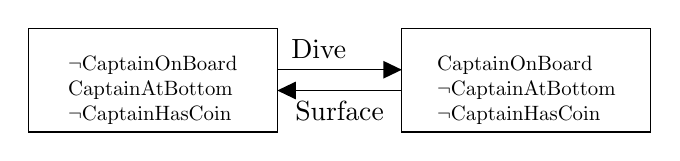
\begin{tikzpicture}[x=0.75pt,y=0.75pt,yscale=-1,xscale=1]
%uncomment if require: \path (0,300); %set diagram left start at 0, and has height of 300

%Shape: Rectangle [id:dp6579865922846719] 
\draw   (340,110) -- (460,110) -- (460,160) -- (340,160) -- cycle ;
%Shape: Rectangle [id:dp9459553670651857] 
\draw   (160,110) -- (280,110) -- (280,160) -- (160,160) -- cycle ;
%Straight Lines [id:da8738748156559979] 
\draw    (280,130) -- (338,130) ;
\draw [shift={(340,130)}, rotate = 180] [fill={rgb, 255:red, 0; green, 0; blue, 0 }  ][line width=0.75]  [draw opacity=0] (8.93,-4.29) -- (0,0) -- (8.93,4.29) -- cycle    ;

%Straight Lines [id:da6875201819727004] 
\draw    (340,140) -- (282,140) ;
\draw [shift={(280,140)}, rotate = 360] [fill={rgb, 255:red, 0; green, 0; blue, 0 }  ][line width=0.75]  [draw opacity=0] (8.93,-4.29) -- (0,0) -- (8.93,4.29) -- cycle    ;


% Text Node
\draw (400,140) node [scale=0.75] [align=left] {CaptainOnBoard\\$\neg$CaptainAtBottom\\$\neg$CaptainHasCoin};
% Text Node
\draw (220,140) node [scale=0.75] [align=left] {$\neg$CaptainOnBoard\\CaptainAtBottom\\$\neg$CaptainHasCoin};
% Text Node
\draw (300,120) node  [align=left] {Dive};
% Text Node
\draw (310,150) node  [align=left] {Surface};


\end{tikzpicture}

\caption{Illustration of the reachable states in the belief state space.}
\label{fig:beliefspace}
\end{figure}


The captain does not know the current location, thus the ship cannot sail anywhere since the \textit{from} value in the precondition is not fulfilled. Therefore the captain can only \textit{Dive} and \textit{Surface} in an infinite loop. See Figure \ref{fig:beliefspace} for an illustration. I have assumed that we still use the closed-world assumptions that $\neg CaptainAtBottom$ and $\neg CaptainHasCoin$.


\subsubsection{Answer to questions}

\begin{itemize}
	\item As given by the PDDL, fluents that are always true include \\ $Next(Bay,White), ~Next(White,Blue), ~Next(Blue,Green)$, \\
    while fluents that are always false include \\
    $Next(Bay,Blue), ~Next(White,Green), ~Next(Bay,Bay)$.
	\item The initial physical state contains 4 states, one for each sea, as we do not know which sea we start in.
	\item There are no plans that lead to satisfaction of the goal, since there is no way of actually sailing between seas (and Picking up the coin from \textit{Blue}). 
	\item As there are no plans that lead to satisfaction of the goal, there is no optimal path. 
\end{itemize}

\subsection{Belief state, with a twist}

\subsubsection{Graph}

\tikzset{every picture/.style={line width=0.75pt}} %set default line width to 0.75pt        

\begin{figure}[h]\centering

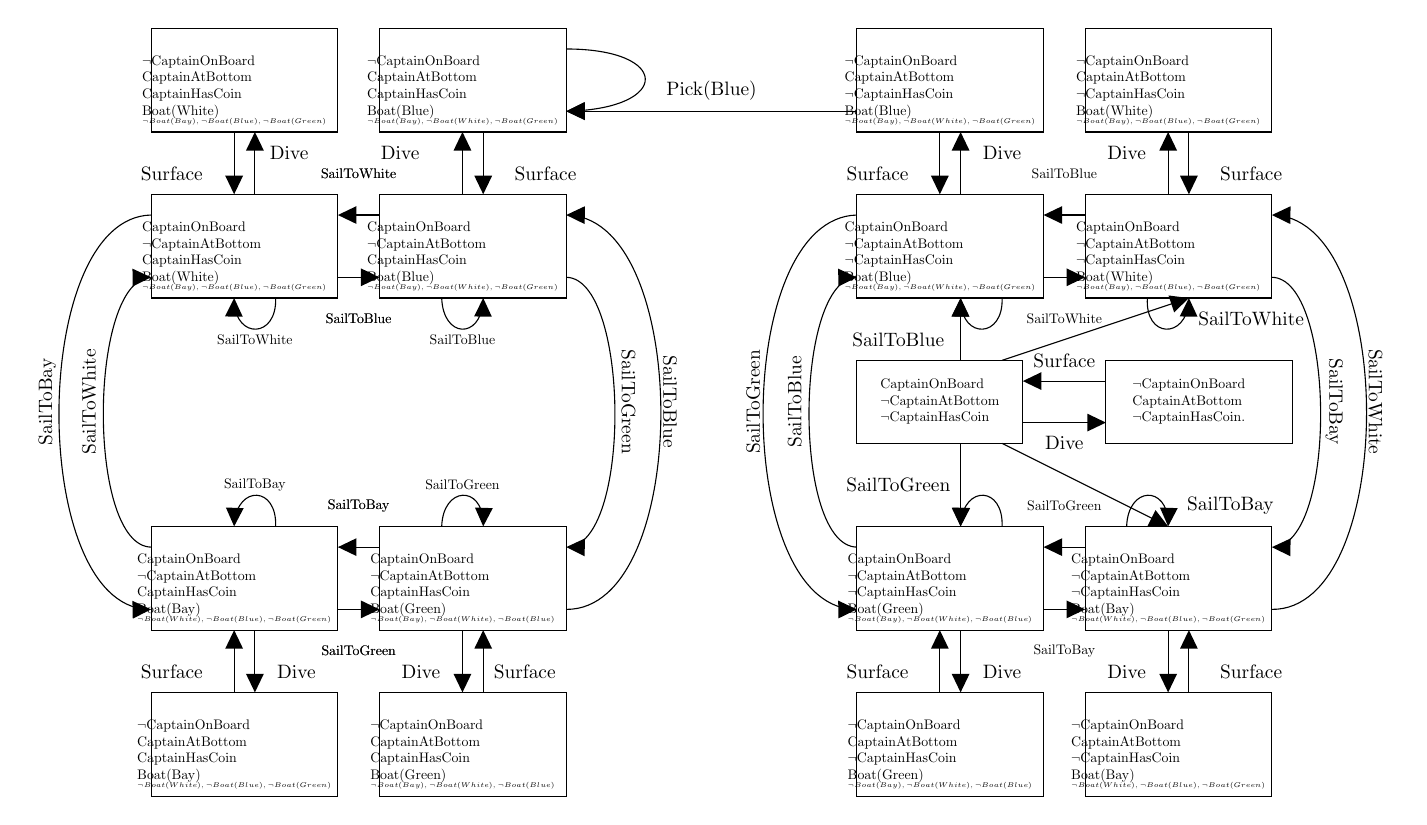
\begin{tikzpicture}[x=0.75pt,y=0.75pt,yscale=-1,xscale=1]
%uncomment if require: \path (0,417.71428298950195); %set diagram left start at 0, and has height of 417.71428298950195

%Shape: Rectangle [id:dp6469361085724255] 
\draw   (400,170) -- (480,170) -- (480,210) -- (400,210) -- cycle ;
%Shape: Rectangle [id:dp5334510482003547] 
\draw   (400,90) -- (490,90) -- (490,140) -- (400,140) -- cycle ;
%Shape: Rectangle [id:dp929040628800839] 
\draw   (400,250) -- (490,250) -- (490,300) -- (400,300) -- cycle ;
%Shape: Rectangle [id:dp4708953694319207] 
\draw   (510,250) -- (600,250) -- (600,300) -- (510,300) -- cycle ;
%Shape: Rectangle [id:dp9354354760243204] 
\draw   (510,90) -- (600,90) -- (600,140) -- (510,140) -- cycle ;
%Shape: Rectangle [id:dp30496763293625406] 
\draw   (400,330) -- (490,330) -- (490,380) -- (400,380) -- cycle ;
%Shape: Rectangle [id:dp2921123123032503] 
\draw   (510,330) -- (600,330) -- (600,380) -- (510,380) -- cycle ;
%Shape: Rectangle [id:dp3506838794551428] 
\draw   (400,10) -- (490,10) -- (490,60) -- (400,60) -- cycle ;
%Shape: Rectangle [id:dp0054106139916383356] 
\draw   (510,10) -- (600,10) -- (600,60) -- (510,60) -- cycle ;
%Curve Lines [id:da5506757826114927] 
\draw    (600,290) .. controls (660.18,290.42) and (660.78,104.21) .. (601.81,100.07) ;
\draw [shift={(600,100)}, rotate = 360.4] [fill={rgb, 255:red, 0; green, 0; blue, 0 }  ][line width=0.75]  [draw opacity=0] (8.93,-4.29) -- (0,0) -- (8.93,4.29) -- cycle    ;

%Curve Lines [id:da6501488519522596] 
\draw    (600,130) .. controls (630.17,130.42) and (631.73,255.28) .. (601.87,259.87) ;
\draw [shift={(600,260)}, rotate = 360.77] [fill={rgb, 255:red, 0; green, 0; blue, 0 }  ][line width=0.75]  [draw opacity=0] (8.93,-4.29) -- (0,0) -- (8.93,4.29) -- cycle    ;

%Curve Lines [id:da37197190565529725] 
\draw    (400,260) .. controls (369.41,259.44) and (369.76,135.54) .. (398.22,130.18) ;
\draw [shift={(400,130)}, rotate = 539.19] [fill={rgb, 255:red, 0; green, 0; blue, 0 }  ][line width=0.75]  [draw opacity=0] (8.93,-4.29) -- (0,0) -- (8.93,4.29) -- cycle    ;

%Curve Lines [id:da202066233535122] 
\draw    (400,100) .. controls (340.39,101.41) and (339.79,286.67) .. (398.21,289.96) ;
\draw [shift={(400,290)}, rotate = 539.5899999999999] [fill={rgb, 255:red, 0; green, 0; blue, 0 }  ][line width=0.75]  [draw opacity=0] (8.93,-4.29) -- (0,0) -- (8.93,4.29) -- cycle    ;

%Straight Lines [id:da47113508051210484] 
\draw    (490,130) -- (508,130) ;
\draw [shift={(510,130)}, rotate = 180] [fill={rgb, 255:red, 0; green, 0; blue, 0 }  ][line width=0.75]  [draw opacity=0] (8.93,-4.29) -- (0,0) -- (8.93,4.29) -- cycle    ;

%Straight Lines [id:da6890984780374445] 
\draw    (490,290) -- (508,290) ;
\draw [shift={(510,290)}, rotate = 180] [fill={rgb, 255:red, 0; green, 0; blue, 0 }  ][line width=0.75]  [draw opacity=0] (8.93,-4.29) -- (0,0) -- (8.93,4.29) -- cycle    ;

%Straight Lines [id:da7563975115906769] 
\draw    (510,260) -- (492,260) ;
\draw [shift={(490,260)}, rotate = 360] [fill={rgb, 255:red, 0; green, 0; blue, 0 }  ][line width=0.75]  [draw opacity=0] (8.93,-4.29) -- (0,0) -- (8.93,4.29) -- cycle    ;

%Straight Lines [id:da051644209394903884] 
\draw    (510,100) -- (492,100) ;
\draw [shift={(490,100)}, rotate = 360] [fill={rgb, 255:red, 0; green, 0; blue, 0 }  ][line width=0.75]  [draw opacity=0] (8.93,-4.29) -- (0,0) -- (8.93,4.29) -- cycle    ;

%Straight Lines [id:da16535456654366176] 
\draw    (450,90) -- (450,62) ;
\draw [shift={(450,60)}, rotate = 450] [fill={rgb, 255:red, 0; green, 0; blue, 0 }  ][line width=0.75]  [draw opacity=0] (8.93,-4.29) -- (0,0) -- (8.93,4.29) -- cycle    ;

%Straight Lines [id:da39127732887891886] 
\draw    (440,60) -- (440,88) ;
\draw [shift={(440,90)}, rotate = 270] [fill={rgb, 255:red, 0; green, 0; blue, 0 }  ][line width=0.75]  [draw opacity=0] (8.93,-4.29) -- (0,0) -- (8.93,4.29) -- cycle    ;

%Straight Lines [id:da410837240925793] 
\draw    (550,90) -- (550,62) ;
\draw [shift={(550,60)}, rotate = 450] [fill={rgb, 255:red, 0; green, 0; blue, 0 }  ][line width=0.75]  [draw opacity=0] (8.93,-4.29) -- (0,0) -- (8.93,4.29) -- cycle    ;

%Straight Lines [id:da3929647730044541] 
\draw    (560,60) -- (560,88) ;
\draw [shift={(560,90)}, rotate = 270] [fill={rgb, 255:red, 0; green, 0; blue, 0 }  ][line width=0.75]  [draw opacity=0] (8.93,-4.29) -- (0,0) -- (8.93,4.29) -- cycle    ;

%Straight Lines [id:da8649566078401985] 
\draw    (560,330) -- (560,302) ;
\draw [shift={(560,300)}, rotate = 450] [fill={rgb, 255:red, 0; green, 0; blue, 0 }  ][line width=0.75]  [draw opacity=0] (8.93,-4.29) -- (0,0) -- (8.93,4.29) -- cycle    ;

%Straight Lines [id:da9759036697509851] 
\draw    (550,300) -- (550,328) ;
\draw [shift={(550,330)}, rotate = 270] [fill={rgb, 255:red, 0; green, 0; blue, 0 }  ][line width=0.75]  [draw opacity=0] (8.93,-4.29) -- (0,0) -- (8.93,4.29) -- cycle    ;

%Straight Lines [id:da8737102932725427] 
\draw    (440,330) -- (440,302) ;
\draw [shift={(440,300)}, rotate = 450] [fill={rgb, 255:red, 0; green, 0; blue, 0 }  ][line width=0.75]  [draw opacity=0] (8.93,-4.29) -- (0,0) -- (8.93,4.29) -- cycle    ;

%Straight Lines [id:da7508496839229659] 
\draw    (450,300) -- (450,328) ;
\draw [shift={(450,330)}, rotate = 270] [fill={rgb, 255:red, 0; green, 0; blue, 0 }  ][line width=0.75]  [draw opacity=0] (8.93,-4.29) -- (0,0) -- (8.93,4.29) -- cycle    ;

%Straight Lines [id:da35528188400016525] 
\draw    (450,170) -- (450,142) ;
\draw [shift={(450,140)}, rotate = 450] [fill={rgb, 255:red, 0; green, 0; blue, 0 }  ][line width=0.75]  [draw opacity=0] (8.93,-4.29) -- (0,0) -- (8.93,4.29) -- cycle    ;

%Straight Lines [id:da28236599470470725] 
\draw    (470,170) -- (558.1,140.63) ;
\draw [shift={(560,140)}, rotate = 521.5699999999999] [fill={rgb, 255:red, 0; green, 0; blue, 0 }  ][line width=0.75]  [draw opacity=0] (8.93,-4.29) -- (0,0) -- (8.93,4.29) -- cycle    ;

%Straight Lines [id:da6272613244836098] 
\draw    (470,210) -- (548.21,249.11) ;
\draw [shift={(550,250)}, rotate = 206.57] [fill={rgb, 255:red, 0; green, 0; blue, 0 }  ][line width=0.75]  [draw opacity=0] (8.93,-4.29) -- (0,0) -- (8.93,4.29) -- cycle    ;

%Straight Lines [id:da31602585714396403] 
\draw    (450,210) -- (450,248) ;
\draw [shift={(450,250)}, rotate = 270] [fill={rgb, 255:red, 0; green, 0; blue, 0 }  ][line width=0.75]  [draw opacity=0] (8.93,-4.29) -- (0,0) -- (8.93,4.29) -- cycle    ;

%Shape: Rectangle [id:dp3873546398816188] 
\draw   (170,10) -- (260,10) -- (260,60) -- (170,60) -- cycle ;
%Straight Lines [id:da4343854691701734] 
\draw    (400,50) -- (262,50) ;
\draw [shift={(260,50)}, rotate = 360] [fill={rgb, 255:red, 0; green, 0; blue, 0 }  ][line width=0.75]  [draw opacity=0] (8.93,-4.29) -- (0,0) -- (8.93,4.29) -- cycle    ;

%Shape: Rectangle [id:dp3895968589306176] 
\draw   (60,90) -- (150,90) -- (150,140) -- (60,140) -- cycle ;
%Shape: Rectangle [id:dp32933245791143073] 
\draw   (60,250) -- (150,250) -- (150,300) -- (60,300) -- cycle ;
%Shape: Rectangle [id:dp7567734820029834] 
\draw   (170,250) -- (260,250) -- (260,300) -- (170,300) -- cycle ;
%Shape: Rectangle [id:dp33389271638136964] 
\draw   (170,90) -- (260,90) -- (260,140) -- (170,140) -- cycle ;
%Shape: Rectangle [id:dp15949017718012182] 
\draw   (170,330) -- (260,330) -- (260,380) -- (170,380) -- cycle ;
%Shape: Rectangle [id:dp4515454317549388] 
\draw   (60,330) -- (150,330) -- (150,380) -- (60,380) -- cycle ;
%Shape: Rectangle [id:dp6984572000018994] 
\draw   (60,10) -- (150,10) -- (150,60) -- (60,60) -- cycle ;
%Curve Lines [id:da7975674908862773] 
\draw    (260,290) .. controls (320.18,290.42) and (320.78,104.21) .. (261.81,100.07) ;
\draw [shift={(260,100)}, rotate = 360.4] [fill={rgb, 255:red, 0; green, 0; blue, 0 }  ][line width=0.75]  [draw opacity=0] (8.93,-4.29) -- (0,0) -- (8.93,4.29) -- cycle    ;

%Curve Lines [id:da9274079526197858] 
\draw    (260,130) .. controls (290.17,130.42) and (291.73,255.28) .. (261.87,259.87) ;
\draw [shift={(260,260)}, rotate = 360.77] [fill={rgb, 255:red, 0; green, 0; blue, 0 }  ][line width=0.75]  [draw opacity=0] (8.93,-4.29) -- (0,0) -- (8.93,4.29) -- cycle    ;

%Curve Lines [id:da6354088193129614] 
\draw    (60,260) .. controls (29.41,259.44) and (29.76,135.54) .. (58.22,130.18) ;
\draw [shift={(60,130)}, rotate = 539.19] [fill={rgb, 255:red, 0; green, 0; blue, 0 }  ][line width=0.75]  [draw opacity=0] (8.93,-4.29) -- (0,0) -- (8.93,4.29) -- cycle    ;

%Curve Lines [id:da7319337089400344] 
\draw    (60,100) .. controls (1.38,101.13) and (0.79,287.36) .. (58.24,289.98) ;
\draw [shift={(60,290)}, rotate = 538.89] [fill={rgb, 255:red, 0; green, 0; blue, 0 }  ][line width=0.75]  [draw opacity=0] (8.93,-4.29) -- (0,0) -- (8.93,4.29) -- cycle    ;

%Straight Lines [id:da5868212582527945] 
\draw    (150,130) -- (168,130) ;
\draw [shift={(170,130)}, rotate = 180] [fill={rgb, 255:red, 0; green, 0; blue, 0 }  ][line width=0.75]  [draw opacity=0] (8.93,-4.29) -- (0,0) -- (8.93,4.29) -- cycle    ;

%Straight Lines [id:da26168424285631775] 
\draw    (150,290) -- (168,290) ;
\draw [shift={(170,290)}, rotate = 180] [fill={rgb, 255:red, 0; green, 0; blue, 0 }  ][line width=0.75]  [draw opacity=0] (8.93,-4.29) -- (0,0) -- (8.93,4.29) -- cycle    ;

%Straight Lines [id:da12065582543044107] 
\draw    (170,260) -- (152,260) ;
\draw [shift={(150,260)}, rotate = 360] [fill={rgb, 255:red, 0; green, 0; blue, 0 }  ][line width=0.75]  [draw opacity=0] (8.93,-4.29) -- (0,0) -- (8.93,4.29) -- cycle    ;

%Straight Lines [id:da7065205441800846] 
\draw    (170,100) -- (152,100) ;
\draw [shift={(150,100)}, rotate = 360] [fill={rgb, 255:red, 0; green, 0; blue, 0 }  ][line width=0.75]  [draw opacity=0] (8.93,-4.29) -- (0,0) -- (8.93,4.29) -- cycle    ;

%Straight Lines [id:da9478193943717605] 
\draw    (110,90) -- (110,62) ;
\draw [shift={(110,60)}, rotate = 450] [fill={rgb, 255:red, 0; green, 0; blue, 0 }  ][line width=0.75]  [draw opacity=0] (8.93,-4.29) -- (0,0) -- (8.93,4.29) -- cycle    ;

%Straight Lines [id:da3874992871555185] 
\draw    (100,60) -- (100,88) ;
\draw [shift={(100,90)}, rotate = 270] [fill={rgb, 255:red, 0; green, 0; blue, 0 }  ][line width=0.75]  [draw opacity=0] (8.93,-4.29) -- (0,0) -- (8.93,4.29) -- cycle    ;

%Straight Lines [id:da05207135034665833] 
\draw    (210,90) -- (210,62) ;
\draw [shift={(210,60)}, rotate = 450] [fill={rgb, 255:red, 0; green, 0; blue, 0 }  ][line width=0.75]  [draw opacity=0] (8.93,-4.29) -- (0,0) -- (8.93,4.29) -- cycle    ;

%Straight Lines [id:da4992021138141254] 
\draw    (220,60) -- (220,88) ;
\draw [shift={(220,90)}, rotate = 270] [fill={rgb, 255:red, 0; green, 0; blue, 0 }  ][line width=0.75]  [draw opacity=0] (8.93,-4.29) -- (0,0) -- (8.93,4.29) -- cycle    ;

%Straight Lines [id:da3168630795732994] 
\draw    (220,330) -- (220,302) ;
\draw [shift={(220,300)}, rotate = 450] [fill={rgb, 255:red, 0; green, 0; blue, 0 }  ][line width=0.75]  [draw opacity=0] (8.93,-4.29) -- (0,0) -- (8.93,4.29) -- cycle    ;

%Straight Lines [id:da43677256989883895] 
\draw    (210,300) -- (210,328) ;
\draw [shift={(210,330)}, rotate = 270] [fill={rgb, 255:red, 0; green, 0; blue, 0 }  ][line width=0.75]  [draw opacity=0] (8.93,-4.29) -- (0,0) -- (8.93,4.29) -- cycle    ;

%Straight Lines [id:da7406878016301024] 
\draw    (100,330) -- (100,302) ;
\draw [shift={(100,300)}, rotate = 450] [fill={rgb, 255:red, 0; green, 0; blue, 0 }  ][line width=0.75]  [draw opacity=0] (8.93,-4.29) -- (0,0) -- (8.93,4.29) -- cycle    ;

%Straight Lines [id:da28929984797263386] 
\draw    (110,300) -- (110,328) ;
\draw [shift={(110,330)}, rotate = 270] [fill={rgb, 255:red, 0; green, 0; blue, 0 }  ][line width=0.75]  [draw opacity=0] (8.93,-4.29) -- (0,0) -- (8.93,4.29) -- cycle    ;

%Curve Lines [id:da6572028568817037] 
\draw    (260,20) .. controls (310.28,20) and (310.78,48.42) .. (261.51,49.96) ;
\draw [shift={(260,50)}, rotate = 358.87] [fill={rgb, 255:red, 0; green, 0; blue, 0 }  ][line width=0.75]  [draw opacity=0] (8.93,-4.29) -- (0,0) -- (8.93,4.29) -- cycle    ;

%Shape: Rectangle [id:dp6493342449594512] 
\draw   (520,170) -- (610,170) -- (610,210) -- (520,210) -- cycle ;
%Straight Lines [id:da40094116174738503] 
\draw    (480,200) -- (518,200) ;
\draw [shift={(520,200)}, rotate = 180] [fill={rgb, 255:red, 0; green, 0; blue, 0 }  ][line width=0.75]  [draw opacity=0] (8.93,-4.29) -- (0,0) -- (8.93,4.29) -- cycle    ;

%Straight Lines [id:da46212510578519383] 
\draw    (520,180) -- (482,180) ;
\draw [shift={(480,180)}, rotate = 360] [fill={rgb, 255:red, 0; green, 0; blue, 0 }  ][line width=0.75]  [draw opacity=0] (8.93,-4.29) -- (0,0) -- (8.93,4.29) -- cycle    ;

%Curve Lines [id:da35738616161543546] 
\draw    (200,140) .. controls (200.68,159.4) and (218.58,159.98) .. (219.92,141.75) ;
\draw [shift={(220,140)}, rotate = 450.86] [fill={rgb, 255:red, 0; green, 0; blue, 0 }  ][line width=0.75]  [draw opacity=0] (8.93,-4.29) -- (0,0) -- (8.93,4.29) -- cycle    ;

%Curve Lines [id:da41952932480623795] 
\draw    (470,140) .. controls (470.68,159.4) and (450.94,159.98) .. (450.03,141.75) ;
\draw [shift={(450,140)}, rotate = 450.86] [fill={rgb, 255:red, 0; green, 0; blue, 0 }  ][line width=0.75]  [draw opacity=0] (8.93,-4.29) -- (0,0) -- (8.93,4.29) -- cycle    ;

%Curve Lines [id:da4880738698754432] 
\draw    (120,140) .. controls (120.68,159.4) and (100.94,159.98) .. (100.03,141.75) ;
\draw [shift={(100,140)}, rotate = 450.86] [fill={rgb, 255:red, 0; green, 0; blue, 0 }  ][line width=0.75]  [draw opacity=0] (8.93,-4.29) -- (0,0) -- (8.93,4.29) -- cycle    ;

%Curve Lines [id:da9458943849186343] 
\draw    (200,250) .. controls (200.68,230.6) and (219.52,230.02) .. (220.01,248.25) ;
\draw [shift={(220,250)}, rotate = 272] [fill={rgb, 255:red, 0; green, 0; blue, 0 }  ][line width=0.75]  [draw opacity=0] (8.93,-4.29) -- (0,0) -- (8.93,4.29) -- cycle    ;

%Curve Lines [id:da15971270644656665] 
\draw    (120,250) .. controls (120.68,230.6) and (101.88,230.02) .. (100.11,248.25) ;
\draw [shift={(100,250)}, rotate = 272] [fill={rgb, 255:red, 0; green, 0; blue, 0 }  ][line width=0.75]  [draw opacity=0] (8.93,-4.29) -- (0,0) -- (8.93,4.29) -- cycle    ;

%Curve Lines [id:da638129549229141] 
\draw    (470,250) .. controls (470.68,230.6) and (451.88,230.02) .. (450.11,248.25) ;
\draw [shift={(450,250)}, rotate = 272] [fill={rgb, 255:red, 0; green, 0; blue, 0 }  ][line width=0.75]  [draw opacity=0] (8.93,-4.29) -- (0,0) -- (8.93,4.29) -- cycle    ;

%Curve Lines [id:da6359245868695376] 
\draw    (530,250) .. controls (530.68,230.6) and (549.52,230.02) .. (550.01,248.25) ;
\draw [shift={(550,250)}, rotate = 272] [fill={rgb, 255:red, 0; green, 0; blue, 0 }  ][line width=0.75]  [draw opacity=0] (8.93,-4.29) -- (0,0) -- (8.93,4.29) -- cycle    ;

%Curve Lines [id:da4187798055415888] 
\draw    (540,140) .. controls (538.74,159.4) and (558.46,159.98) .. (559.92,141.75) ;
\draw [shift={(560,140)}, rotate = 450.86] [fill={rgb, 255:red, 0; green, 0; blue, 0 }  ][line width=0.75]  [draw opacity=0] (8.93,-4.29) -- (0,0) -- (8.93,4.29) -- cycle    ;


% Text Node
\draw (440,120) node [scale=0.5] [align=left] {CaptainOnBoard\\$\neg$CaptainAtBottom\\$\neg$CaptainHasCoin\\Boat(Blue)\\[-6pt]\tiny$\neg Boat(Bay), \neg Boat(White), \neg Boat(Green)$};
% Text Node
\draw (440,190) node [scale=0.5] [align=left] {CaptainOnBoard\\$\neg$CaptainAtBottom\\$\neg$CaptainHasCoin};
% Text Node
\draw (440,280) node [scale=0.5] [align=left] {CaptainOnBoard\\$\neg$CaptainAtBottom\\$\neg$CaptainHasCoin\\Boat(Green)\\[-6pt]\tiny$\neg Boat(Bay), \neg Boat(White), \neg Boat(Blue)$};
% Text Node
\draw (550,280) node [scale=0.5] [align=left] {CaptainOnBoard\\$\neg$CaptainAtBottom\\$\neg$CaptainHasCoin\\Boat(Bay)\\[-6pt]\tiny$\neg Boat(White), \neg Boat(Blue), \neg Boat(Green)$};
% Text Node
\draw (550,120) node [scale=0.5] [align=left] {CaptainOnBoard\\$\neg$CaptainAtBottom\\$\neg$CaptainHasCoin\\Boat(White)\\[-6pt]\tiny$\neg Boat(Bay), \neg Boat(Blue), \neg Boat(Green)$};
% Text Node
\draw (440,360) node [scale=0.5] [align=left] {$\neg$CaptainOnBoard\\CaptainAtBottom\\$\neg$CaptainHasCoin\\Boat(Green)\\[-6pt]\tiny$\neg Boat(Bay), \neg Boat(White), \neg Boat(Blue)$};
% Text Node
\draw (550,360) node [scale=0.5] [align=left] {$\neg$CaptainOnBoard\\CaptainAtBottom\\$\neg$CaptainHasCoin\\Boat(Bay)\\[-6pt]\tiny$\neg Boat(White), \neg Boat(Blue), \neg Boat(Green)$};
% Text Node
\draw (440,40) node [scale=0.5] [align=left] {$\neg$CaptainOnBoard\\CaptainAtBottom\\$\neg$CaptainHasCoin\\Boat(Blue)\\[-6pt]\tiny$\neg Boat(Bay), \neg Boat(White), \neg Boat(Green)$};
% Text Node
\draw (550,40) node [scale=0.5] [align=left] {$\neg$CaptainOnBoard\\CaptainAtBottom\\$\neg$CaptainHasCoin\\Boat(White)\\[-6pt]\tiny$\neg Boat(Bay), \neg Boat(Blue), \neg Boat(Green)$};
% Text Node
\draw (470,70) node [scale=0.7] [align=left] {Dive};
% Text Node
\draw (530,70) node [scale=0.7] [align=left] {Dive};
% Text Node
\draw (530,320) node [scale=0.7] [align=left] {Dive};
% Text Node
\draw (470,320) node [scale=0.7] [align=left] {Dive};
% Text Node
\draw (410,80) node [scale=0.7] [align=left] {Surface};
% Text Node
\draw (590,80) node [scale=0.7] [align=left] {Surface};
% Text Node
\draw (590,320) node [scale=0.7] [align=left] {Surface};
% Text Node
\draw (410,320) node [scale=0.7] [align=left] {Surface};
% Text Node
\draw (210,40) node [scale=0.5] [align=left] {$\neg$CaptainOnBoard\\CaptainAtBottom\\CaptainHasCoin\\Boat(Blue)\\[-6pt]\tiny$\neg Boat(Bay), \neg Boat(White), \neg Boat(Green)$};
% Text Node
\draw (580,240) node [scale=0.7] [align=left] {SailToBay};
% Text Node
\draw (630,190) node [scale=0.7,rotate=-90] [align=left] {SailToBay};
% Text Node
\draw (500,310) node [scale=0.5] [align=left] {SailToBay};
% Text Node
\draw (500,240) node [scale=0.5] [align=left] {SailToGreen};
% Text Node
\draw (500,150) node [scale=0.5] [align=left] {SailToWhite};
% Text Node
\draw (500,80) node [scale=0.5] [align=left] {SailToBlue};
% Text Node
\draw (650,190) node [scale=0.7,rotate=-90] [align=left] {SailToWhite};
% Text Node
\draw (590,150) node [scale=0.7] [align=left] {SailToWhite};
% Text Node
\draw (420,160) node [scale=0.7] [align=left] {SailToBlue};
% Text Node
\draw (370,190) node [scale=0.7,rotate=-270] [align=left] {SailToBlue};
% Text Node
\draw (350,190) node [scale=0.7,rotate=-270] [align=left] {SailToGreen};
% Text Node
\draw (420,230) node [scale=0.7] [align=left] {SailToGreen};
% Text Node
\draw (330,40) node [scale=0.7] [align=left] {Pick(Blue)};
% Text Node
\draw (210,120) node [scale=0.5] [align=left] {CaptainOnBoard\\$\neg$CaptainAtBottom\\CaptainHasCoin\\Boat(Blue)\\[-6pt]\tiny$\neg Boat(Bay), \neg Boat(White), \neg Boat(Green)$};
% Text Node
\draw (210,280) node [scale=0.5] [align=left] {CaptainOnBoard\\$\neg$CaptainAtBottom\\CaptainHasCoin\\Boat(Green)\\[-6pt]\tiny$\neg Boat(Bay), \neg Boat(White), \neg Boat(Blue)$};
% Text Node
\draw (100,280) node [scale=0.5] [align=left] {CaptainOnBoard\\$\neg$CaptainAtBottom\\CaptainHasCoin\\Boat(Bay)\\[-6pt]\tiny$\neg Boat(White), \neg Boat(Blue), \neg Boat(Green)$};
% Text Node
\draw (100,120) node [scale=0.5] [align=left] {CaptainOnBoard\\$\neg$CaptainAtBottom\\CaptainHasCoin\\Boat(White)\\[-6pt]\tiny$\neg Boat(Bay), \neg Boat(Blue), \neg Boat(Green)$};
% Text Node
\draw (210,360) node [scale=0.5] [align=left] {$\neg$CaptainOnBoard\\CaptainAtBottom\\CaptainHasCoin\\Boat(Green)\\[-6pt]\tiny$\neg Boat(Bay), \neg Boat(White), \neg Boat(Blue)$};
% Text Node
\draw (100,360) node [scale=0.5] [align=left] {$\neg$CaptainOnBoard\\CaptainAtBottom\\CaptainHasCoin\\Boat(Bay)\\[-6pt]\tiny$\neg Boat(White), \neg Boat(Blue), \neg Boat(Green)$};
% Text Node
\draw (100,40) node [scale=0.5] [align=left] {$\neg$CaptainOnBoard\\CaptainAtBottom\\CaptainHasCoin\\Boat(White)\\[-6pt]\tiny$\neg Boat(Bay), \neg Boat(Blue), \neg Boat(Green)$};
% Text Node
\draw (126.5,70) node [scale=0.7] [align=left] {Dive};
% Text Node
\draw (180,70) node [scale=0.7] [align=left] {Dive};
% Text Node
\draw (190,320) node [scale=0.7] [align=left] {Dive};
% Text Node
\draw (130,320) node [scale=0.7] [align=left] {Dive};
% Text Node
\draw (70,80) node [scale=0.7] [align=left] {Surface};
% Text Node
\draw (250,80) node [scale=0.7] [align=left] {Surface};
% Text Node
\draw (240,320) node [scale=0.7] [align=left] {Surface};
% Text Node
\draw (70,320) node [scale=0.7] [align=left] {Surface};
% Text Node
\draw (10,190) node [scale=0.7,rotate=-270] [align=left] {SailToBay};
% Text Node
\draw (160,240) node [scale=0.5] [align=left] {SailToBay};
% Text Node
\draw (160,310) node [scale=0.5] [align=left] {SailToGreen};
% Text Node
\draw (160,80) node [scale=0.5] [align=left] {SailToWhite};
% Text Node
\draw (160,150) node [scale=0.5] [align=left] {SailToBlue};
% Text Node
\draw (30,190) node [scale=0.7,rotate=-270] [align=left] {SailToWhite};
% Text Node
\draw (310,190) node [scale=0.7,rotate=-90] [align=left] {SailToBlue};
% Text Node
\draw (290,190) node [scale=0.7,rotate=-90] [align=left] {SailToGreen};
% Text Node
\draw (560,190) node [scale=0.5] [align=left] {$\neg$CaptainOnBoard\\CaptainAtBottom\\$\neg$CaptainHasCoin.};
% Text Node
\draw (500,210) node [scale=0.7] [align=left] {Dive};
% Text Node
\draw (500,170) node [scale=0.7] [align=left] {Surface};
% Text Node
\draw (160,240) node [scale=0.5] [align=left] {SailToBay};
% Text Node
\draw (160,310) node [scale=0.5] [align=left] {SailToGreen};
% Text Node
\draw (160,80) node [scale=0.5] [align=left] {SailToWhite};
% Text Node
\draw (160,150) node [scale=0.5] [align=left] {SailToBlue};
% Text Node
\draw (210,230) node [scale=0.5] [align=left] {SailToGreen};
% Text Node
\draw (110,230) node [scale=0.5] [align=left] {SailToBay};
% Text Node
\draw (210,160) node [scale=0.5] [align=left] {SailToBlue};
% Text Node
\draw (110,160) node [scale=0.5] [align=left] {SailToWhite};


\end{tikzpicture}

    \caption{Belief state space with modified SailTo actions}
\label{fig:beliefstatemodified}
\end{figure}

As soon as the captain sails to either se from the initial state, we will be certain of where we are, and can use the same method as the fully observable states, ie sailing wherever we want. Please see Figure \ref{fig:beliefstatemodified}. Just as in the previous problem I assume that we still use the closed-world assumptions that $\neg CaptainAtBottom$ and $\neg CaptainHasCoin$. Should that not be the case, then the drawn graph would be much larger.

\subsubsection{Answer to questions}

\begin{itemize}
	\item The initial physical state still contains 4 states, since there are still 4 possible seas that the ship may be located at.
	\item There are still an infinite number of plans leading to satisfaction of the goal, as it is still possible to get caught in infinite loops of jumping back and forth between seas. 
	\item The most optimal plan is now only 5 steps, because can proceed directly from sea to sea without going through unneccessary seas. The most optimal path is
	\begin{equation}
		SailToBlue ~\rightarrow~ Dive ~\rightarrow~ Pick(Blue) ~\rightarrow~ Surface ~\rightarrow~ SailToBay
	\end{equation}
\end{itemize}

\subsection{State space with Percept}

\subsubsection{Graph}

\tikzset{every picture/.style={line width=0.75pt}} %set default line width to 0.75pt        

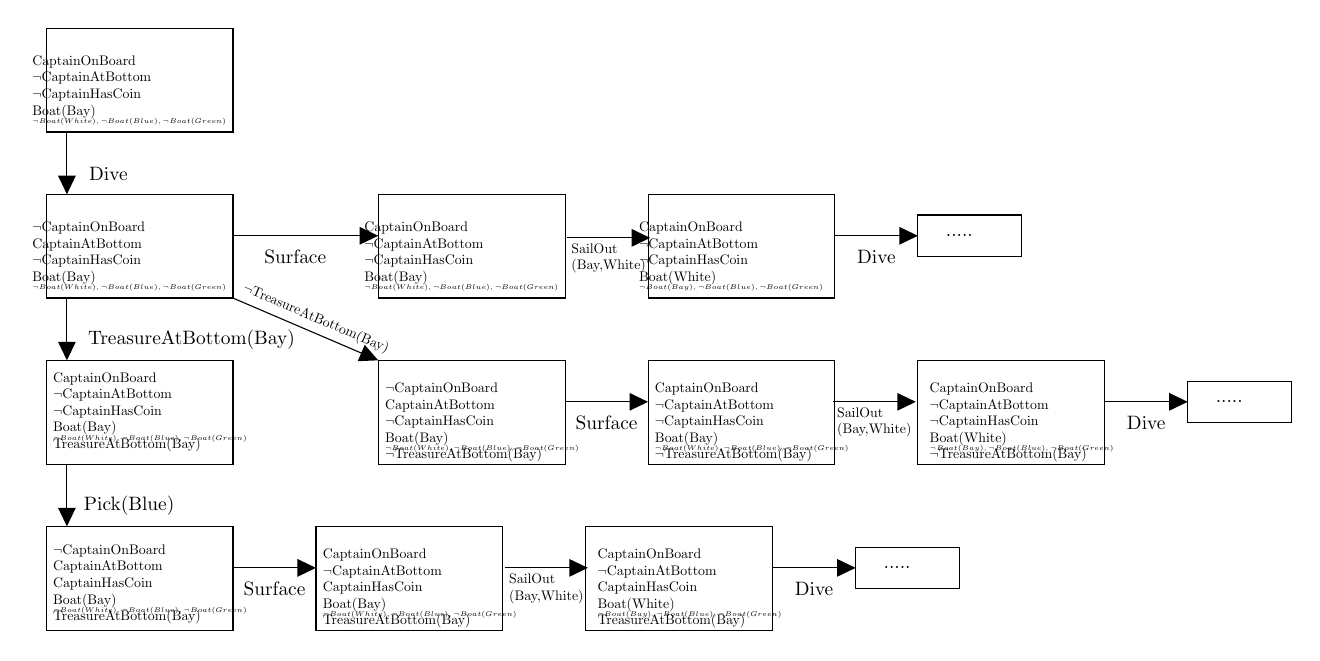
\begin{tikzpicture}[x=0.75pt,y=0.75pt,yscale=-1,xscale=1]
%uncomment if require: \path (0,300); %set diagram left start at 0, and has height of 300

%Shape: Rectangle [id:dp18548487107819578] 
\draw   (30,80) -- (120,80) -- (120,130) -- (30,130) -- cycle ;
%Shape: Rectangle [id:dp12296322805024285] 
\draw   (190,80) -- (280,80) -- (280,130) -- (190,130) -- cycle ;
%Straight Lines [id:da978921004144016] 
\draw    (120,100) -- (188,100) ;
\draw [shift={(190,100)}, rotate = 180] [fill={rgb, 255:red, 0; green, 0; blue, 0 }  ][line width=0.75]  [draw opacity=0] (8.93,-4.29) -- (0,0) -- (8.93,4.29) -- cycle    ;

%Straight Lines [id:da3441657660866113] 
\draw    (40,130) -- (40,158) ;
\draw [shift={(40,160)}, rotate = 270] [fill={rgb, 255:red, 0; green, 0; blue, 0 }  ][line width=0.75]  [draw opacity=0] (8.93,-4.29) -- (0,0) -- (8.93,4.29) -- cycle    ;

%Shape: Rectangle [id:dp9800622932355725] 
\draw   (30,160) -- (120,160) -- (120,210) -- (30,210) -- cycle ;
%Straight Lines [id:da842649655354857] 
\draw    (40,210) -- (40,238) ;
\draw [shift={(40,240)}, rotate = 270] [fill={rgb, 255:red, 0; green, 0; blue, 0 }  ][line width=0.75]  [draw opacity=0] (8.93,-4.29) -- (0,0) -- (8.93,4.29) -- cycle    ;

%Shape: Rectangle [id:dp2716850055211626] 
\draw   (30,240) -- (120,240) -- (120,290) -- (30,290) -- cycle ;
%Shape: Rectangle [id:dp14804048012746995] 
\draw   (160,240) -- (250,240) -- (250,290) -- (160,290) -- cycle ;
%Straight Lines [id:da32169665821669113] 
\draw    (120,260) -- (158,260) ;
\draw [shift={(160,260)}, rotate = 180] [fill={rgb, 255:red, 0; green, 0; blue, 0 }  ][line width=0.75]  [draw opacity=0] (8.93,-4.29) -- (0,0) -- (8.93,4.29) -- cycle    ;

%Shape: Rectangle [id:dp1836254987883852] 
\draw   (190,160) -- (280,160) -- (280,210) -- (190,210) -- cycle ;
%Straight Lines [id:da9265917865326245] 
\draw    (120,130) -- (188.16,159.21) ;
\draw [shift={(190,160)}, rotate = 203.2] [fill={rgb, 255:red, 0; green, 0; blue, 0 }  ][line width=0.75]  [draw opacity=0] (8.93,-4.29) -- (0,0) -- (8.93,4.29) -- cycle    ;

%Shape: Rectangle [id:dp6645619889461027] 
\draw   (320,160) -- (410,160) -- (410,210) -- (320,210) -- cycle ;
%Straight Lines [id:da5122989254835038] 
\draw    (280,180) -- (318,180) ;
\draw [shift={(320,180)}, rotate = 180] [fill={rgb, 255:red, 0; green, 0; blue, 0 }  ][line width=0.75]  [draw opacity=0] (8.93,-4.29) -- (0,0) -- (8.93,4.29) -- cycle    ;

%Shape: Rectangle [id:dp9075905103861217] 
\draw   (450,160) -- (540,160) -- (540,210) -- (450,210) -- cycle ;
%Straight Lines [id:da3982801378128855] 
\draw    (281,101) -- (319,101) ;
\draw [shift={(321,101)}, rotate = 180] [fill={rgb, 255:red, 0; green, 0; blue, 0 }  ][line width=0.75]  [draw opacity=0] (8.93,-4.29) -- (0,0) -- (8.93,4.29) -- cycle    ;

%Shape: Rectangle [id:dp5147590830539686] 
\draw   (320,80) -- (410,80) -- (410,130) -- (320,130) -- cycle ;
%Straight Lines [id:da8246156137716087] 
\draw    (410,100) -- (448,100) ;
\draw [shift={(450,100)}, rotate = 180] [fill={rgb, 255:red, 0; green, 0; blue, 0 }  ][line width=0.75]  [draw opacity=0] (8.93,-4.29) -- (0,0) -- (8.93,4.29) -- cycle    ;

%Shape: Rectangle [id:dp04849336602847765] 
\draw   (450,90) -- (500,90) -- (500,110) -- (450,110) -- cycle ;
%Straight Lines [id:da3609077475442386] 
\draw    (409,180) -- (447,180) ;
\draw [shift={(449,180)}, rotate = 180] [fill={rgb, 255:red, 0; green, 0; blue, 0 }  ][line width=0.75]  [draw opacity=0] (8.93,-4.29) -- (0,0) -- (8.93,4.29) -- cycle    ;

%Straight Lines [id:da46816058551394835] 
\draw    (540,180) -- (578,180) ;
\draw [shift={(580,180)}, rotate = 180] [fill={rgb, 255:red, 0; green, 0; blue, 0 }  ][line width=0.75]  [draw opacity=0] (8.93,-4.29) -- (0,0) -- (8.93,4.29) -- cycle    ;

%Shape: Rectangle [id:dp7516378886244535] 
\draw   (580,170) -- (630,170) -- (630,190) -- (580,190) -- cycle ;
%Straight Lines [id:da6555361699444586] 
\draw    (251,260) -- (289,260) ;
\draw [shift={(291,260)}, rotate = 180] [fill={rgb, 255:red, 0; green, 0; blue, 0 }  ][line width=0.75]  [draw opacity=0] (8.93,-4.29) -- (0,0) -- (8.93,4.29) -- cycle    ;

%Shape: Rectangle [id:dp0034013087097193306] 
\draw   (290,240) -- (380,240) -- (380,290) -- (290,290) -- cycle ;
%Straight Lines [id:da48254825135501567] 
\draw    (380,260) -- (418,260) ;
\draw [shift={(420,260)}, rotate = 180] [fill={rgb, 255:red, 0; green, 0; blue, 0 }  ][line width=0.75]  [draw opacity=0] (8.93,-4.29) -- (0,0) -- (8.93,4.29) -- cycle    ;

%Shape: Rectangle [id:dp11744584106597089] 
\draw   (420,250) -- (470,250) -- (470,270) -- (420,270) -- cycle ;
%Shape: Rectangle [id:dp40733763711640547] 
\draw   (30,0) -- (120,0) -- (120,50) -- (30,50) -- cycle ;
%Straight Lines [id:da8605160116804946] 
\draw    (40,50) -- (40,78) ;
\draw [shift={(40,80)}, rotate = 270] [fill={rgb, 255:red, 0; green, 0; blue, 0 }  ][line width=0.75]  [draw opacity=0] (8.93,-4.29) -- (0,0) -- (8.93,4.29) -- cycle    ;


% Text Node
\draw (70,110) node [scale=0.5] [align=left] {$\neg$CaptainOnBoard\\CaptainAtBottom\\$\neg$CaptainHasCoin\\Boat(Bay)\\[-6pt]\tiny$\neg Boat(White), \neg Boat(Blue), \neg Boat(Green)$};
% Text Node
\draw (230,110) node [scale=0.5] [align=left] {CaptainOnBoard\\$\neg$CaptainAtBottom\\$\neg$CaptainHasCoin\\Boat(Bay)\\[-6pt]\tiny$\neg Boat(White), \neg Boat(Blue), \neg Boat(Green)$};
% Text Node
\draw (300,190) node [scale=0.7] [align=left] {Surface};
% Text Node
\draw (80,185) node [scale=0.5] [align=left] {CaptainOnBoard\\$\neg$CaptainAtBottom\\$\neg$CaptainHasCoin\\Boat(Bay)\\[-6pt]\tiny$\neg Boat(White), \neg Boat(Blue), \neg Boat(Green)$\\[-6pt]TreasureAtBottom(Bay)};
% Text Node
\draw (100,150) node [scale=0.7] [align=left] {TreasureAtBottom(Bay)};
% Text Node
\draw (70,230) node [scale=0.7] [align=left] {Pick(Blue)};
% Text Node
\draw (80,268) node [scale=0.5] [align=left] {$\neg$CaptainOnBoard\\CaptainAtBottom\\CaptainHasCoin\\Boat(Bay)\\[-6pt]\tiny$\neg Boat(White), \neg Boat(Blue), \neg Boat(Green)$\\[-6pt]TreasureAtBottom(Bay)};
% Text Node
\draw (210,270) node [scale=0.5] [align=left] {CaptainOnBoard\\$\neg$CaptainAtBottom\\CaptainHasCoin\\Boat(Bay)\\[-6pt]\tiny$\neg Boat(White), \neg Boat(Blue), \neg Boat(Green)$\\[-6pt]TreasureAtBottom(Bay)};
% Text Node
\draw (140,270) node [scale=0.7] [align=left] {Surface};
% Text Node
\draw (240,190) node [scale=0.5] [align=left] {$\neg$CaptainOnBoard\\CaptainAtBottom\\$\neg$CaptainHasCoin\\Boat(Bay)\\[-6pt]\tiny$\neg Boat(White), \neg Boat(Blue), \neg Boat(Green)$\\[-6pt]$\neg$TreasureAtBottom(Bay)};
% Text Node
\draw (160,140) node [scale=0.5,rotate=-23] [align=left] {$\neg$TreasureAtBottom(Bay)};
% Text Node
\draw (370,190) node [scale=0.5] [align=left] {CaptainOnBoard\\$\neg$CaptainAtBottom\\$\neg$CaptainHasCoin\\Boat(Bay)\\[-6pt]\tiny$\neg Boat(White), \neg Boat(Blue), \neg Boat(Green)$\\[-6pt]$\neg$TreasureAtBottom(Bay)};
% Text Node
\draw (301,111) node [scale=0.5] [align=left] {SailOut\\(Bay,White)};
% Text Node
\draw (500,190) node [scale=0.5] [align=left] {CaptainOnBoard\\$\neg$CaptainAtBottom\\$\neg$CaptainHasCoin\\Boat(White)\\[-6pt]\tiny$\neg Boat(Bay), \neg Boat(Blue), \neg Boat(Green)$\\[-6pt]$\neg$TreasureAtBottom(Bay)};
% Text Node
\draw (150,110) node [scale=0.7] [align=left] {Surface};
% Text Node
\draw (360,110) node [scale=0.5] [align=left] {CaptainOnBoard\\$\neg$CaptainAtBottom\\$\neg$CaptainHasCoin\\Boat(White)\\[-6pt]\tiny$\neg Boat(Bay), \neg Boat(Blue), \neg Boat(Green)$};
% Text Node
\draw (430,110) node [scale=0.7] [align=left] {Dive};
% Text Node
\draw (470,100) node [scale=0.7] [align=left] {.....};
% Text Node
\draw (429,190) node [scale=0.5] [align=left] {SailOut\\(Bay,White)};
% Text Node
\draw (560,190) node [scale=0.7] [align=left] {Dive};
% Text Node
\draw (600,180) node [scale=0.7] [align=left] {.....};
% Text Node
\draw (271,270) node [scale=0.5] [align=left] {SailOut\\(Bay,White)};
% Text Node
\draw (340,270) node [scale=0.5] [align=left] {CaptainOnBoard\\$\neg$CaptainAtBottom\\CaptainHasCoin\\Boat(White)\\[-6pt]\tiny$\neg Boat(Bay), \neg Boat(Blue), \neg Boat(Green)$\\[-6pt]TreasureAtBottom(Bay)};
% Text Node
\draw (400,270) node [scale=0.7] [align=left] {Dive};
% Text Node
\draw (440,260) node [scale=0.7] [align=left] {.....};
% Text Node
\draw (70,30) node [scale=0.5] [align=left] {CaptainOnBoard\\$\neg$CaptainAtBottom\\$\neg$CaptainHasCoin\\Boat(Bay)\\[-6pt]\tiny$\neg Boat(White), \neg Boat(Blue), \neg Boat(Green)$};
% Text Node
\draw (60,70) node [scale=0.7] [align=left] {Dive};
\end{tikzpicture}

In essence, the captain can still dive at every sea, but when the captain dives at a sea he has not dived at before, the captain can choose to either \textit{Surface} immediately, or perceive whether there is a treasure there or not. This effectively splits into 3 subtrees:

\begin{itemize}
	\item One with the same information as before, the captain surfaces, and can either dive immediately again, or keep sailing. Rinse and repeat.
	\item If \textit{Perceive} is executed, we will end up with more information, either \textit{TreasureAtBottom(at)} or \textit{$\neg$TreasureAtBottom(at)}, and the now known fluent will result in 2 new subtrees where this information is known. This process is repeated at each diving point, leading to a lot of subtrees. Of course subtrees can be connected to each other if for instance if \textit{TreasureAtBottom(Blue)} and \textit{TreasureAtBottom(White)} are Perceived in one subtree (in that order), and another Perceives them in opposite order; the information gained is still the same. 
\end{itemize}



\subsubsection{Contingent plan}


\begin{lstlisting}
//Assume initial sea is Bay
Dive();
if (TreasureAtBottom(Bay)) {
    Pick(Bay); 
    Surface();
    return;
}
else {
    Surface();
    SailOut(Bay,White);
    Dive();
    if (TreasureAtBottom(White)) {
        Pick(White); 
        Surface();
    }
    else {
        Surface();
        SailOut(White,Blue);
        Dive();
        if (TreasureAtBottom(Blue)) {
            Pick(Blue); 
            Surface();
        }
        else {
            Surface();
            SailOut(Blue,Green);
            Dive(); 
            if (TreasureAtBottom(Green)) { 	// Unnecessary
                Pick(Green); 
                Surface();
            }                               // Unnecessary
            else {                          // Unnecessary
                Surface();   
                NoOp();                     // Unnecessary
            }                               // Unnecessary
            SailIn(Green,Blue);
        }
        SailIn(Blue,White);
    }
    SailIn(White,Bay);
    return;
}




\end{lstlisting}

The lines marked as Unnecessary do not apply if the algorithm works under the assumption that there is a treasure, and that there is only one treasure in our world (because the algorithm \textit{will} find a treasure somewhere). \\

\subsection{B-level questions}

\begin{itemize}
    \item If we compare the size of the state space graph in Figure \ref{fig:statespace} with the belief state space graph in Figure \ref{fig:beliefstatemodified}, I we see that in these specific domains the belief state space graph will always be larger than the state space graph. This is because the belief state graph will always have an initial state where the location is unknown, and one action is required to determine the current location/sea, thus one extra node will always exist in the belief space graph. However if we instead consider the first sensorless case which has only 2 reachable states from the initial state (initial state included) as seen in Figure \ref{fig:beliefspace}, we see that the belief state space can indeed be smaller than the state space state. Its all dependent on how the domain is defined. 
    \item Consider the initial state in the sensorless case in Figure \ref{fig:beliefstatemodified}, where there are 3 fluents, and the initial state in the fully observable case in Figure \ref{fig:statespace} where there are only 2 explicitly listed fluents. This would suggest that the size of the representation of the fully observable case is larger than the sensorless case equivalent. However imagine that we are in a PDDL domain where there is no coin, and the captain cannot dive, ie the fluents \textit{CaptainAtBottom} and \textit{CaptainHasCoin} do not exist. Then we have the opposite space size relation when the size of the representation of the fully observable case is \textit{smaller} than the sensorless equivalent. I thus must conclude that the size relation between the fully observable and sensorless cases is not a oneway street. It is dependent on how many negative fluents are known in the initial state (and also on how the domain is defined).
    (This assumes that the fully observable case is a closed world, and the sensorless case an open world)
\end{itemize}

\section{Exercise 4}

The following environment was given:
\begin{figure}[h]\centering
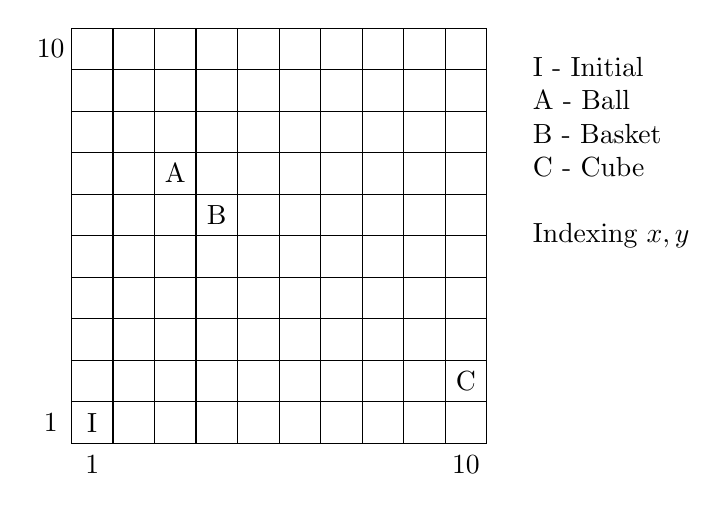
\begin{tikzpicture}[x=0.75pt,y=0.75pt,yscale=-1,xscale=1]
%uncomment if require: \path (0,300); %set diagram left start at 0, and has height of 300

%Shape: Rectangle [id:dp5158705747440835] 
\draw   (200,40) -- (400,40) -- (400,240) -- (200,240) -- cycle ;
%Straight Lines [id:da873350068948654] 
\draw    (200,60) -- (400,60) ;


%Straight Lines [id:da9621658346246118] 
\draw    (200,80) -- (400,80) ;


%Straight Lines [id:da9621372725266528] 
\draw    (200,100) -- (400,100) ;


%Straight Lines [id:da7266368187779007] 
\draw    (200,220) -- (400,220) ;


%Straight Lines [id:da9054330596868856] 
\draw    (200,120) -- (400,120) ;


%Straight Lines [id:da096808959836727] 
\draw    (200,140) -- (400,140) ;


%Straight Lines [id:da3874206218581324] 
\draw    (200,160) -- (400,160) ;


%Straight Lines [id:da32721915323855355] 
\draw    (200,180) -- (400,180) ;


%Straight Lines [id:da8667528343712168] 
\draw    (200,200) -- (400,200) ;


%Straight Lines [id:da6932984736624912] 
\draw    (220,40) -- (220,240) ;


%Straight Lines [id:da671117447971475] 
\draw    (240,40) -- (240,240) ;


%Straight Lines [id:da5139914329608479] 
\draw    (260,40) -- (260,240) ;


%Straight Lines [id:da5338407156452671] 
\draw    (280,40) -- (280,240) ;


%Straight Lines [id:da981027337925209] 
\draw    (300,40) -- (300,240) ;


%Straight Lines [id:da30845575411543846] 
\draw    (320,40) -- (320,240) ;


%Straight Lines [id:da06064324564669543] 
\draw    (340,40) -- (340,240) ;


%Straight Lines [id:da3952658825574047] 
\draw    (360,40) -- (360,240) ;


%Straight Lines [id:da9615274747782987] 
\draw    (380,40) -- (380,240) ;



% Text Node
\draw (210,250) node  [align=left] {1};
% Text Node
\draw (190,230) node  [align=left] {1};
% Text Node
\draw (390,250) node  [align=left] {10};
% Text Node
\draw (190,50) node  [align=left] {10};
% Text Node
\draw (250,110) node  [align=left] {A};
% Text Node
\draw (270,130) node  [align=left] {B};
% Text Node
\draw (390,210) node  [align=left] {};
% Text Node
\draw (210,230) node  [align=left] {I};
% Text Node
\draw (390,210) node  [align=left] {C};
% Text Node
\draw (460,100) node  [align=left] {I - Initial\\A - Ball\\B - Basket\\C - Cube\\\\Indexing $\displaystyle x,y$};


\end{tikzpicture}

    \caption{Illustration of the robot world}
    \label{fig:robotworld}
\end{figure}
	
\subsection{C-level}

See Figure \ref{fig:robotheuristics} for graphical representation.

\tikzset{every picture/.style={line width=0.75pt}} %set default line width to 0.75pt       

\begin{figure}[h]\centering

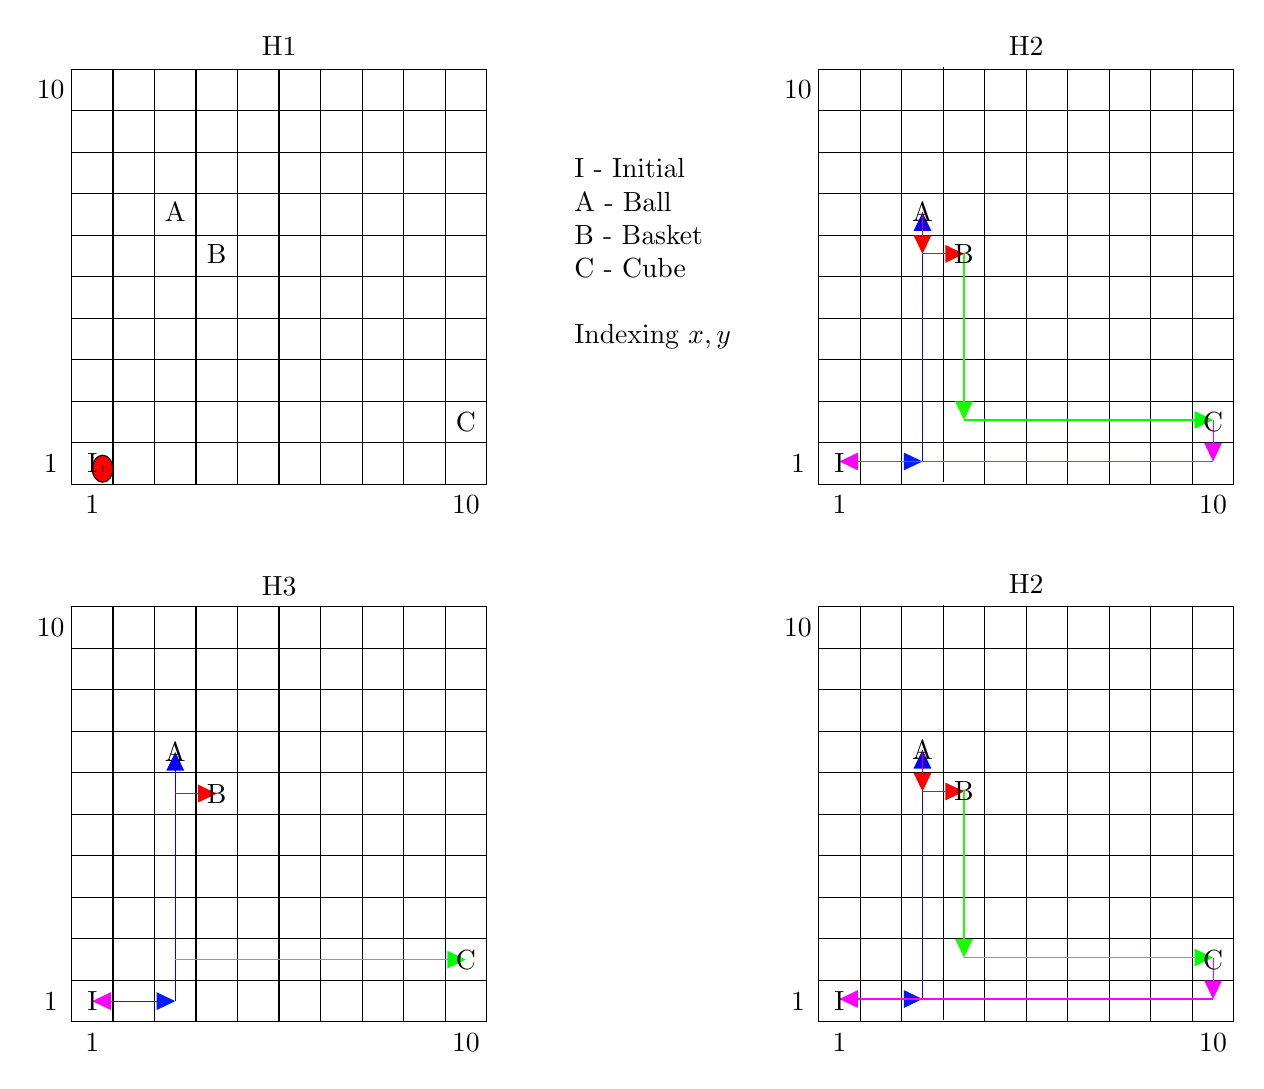
\begin{tikzpicture}[x=0.75pt,y=0.75pt,yscale=-1,xscale=1]
%uncomment if require: \path (0,530.8000030517578); %set diagram left start at 0, and has height of 530.8000030517578

%Shape: Rectangle [id:dp3037294548735383] 
\draw   (50,41) -- (250,41) -- (250,241) -- (50,241) -- cycle ;
%Straight Lines [id:da1043242098308419] 
\draw    (50,61) -- (250,61) ;


%Straight Lines [id:da7378721006745066] 
\draw    (50,81) -- (250,81) ;


%Straight Lines [id:da4691966880170484] 
\draw    (50,101) -- (250,101) ;


%Straight Lines [id:da14745337124638103] 
\draw    (50,221) -- (250,221) ;


%Straight Lines [id:da2798750811444377] 
\draw    (50,121) -- (250,121) ;


%Straight Lines [id:da4595387420664372] 
\draw    (50,141) -- (250,141) ;


%Straight Lines [id:da22269796396357577] 
\draw    (50,161) -- (250,161) ;


%Straight Lines [id:da7036260442545095] 
\draw    (50,181) -- (250,181) ;


%Straight Lines [id:da40734651005178324] 
\draw    (50,201) -- (250,201) ;


%Straight Lines [id:da5250208897506285] 
\draw    (70,41) -- (70,241) ;


%Straight Lines [id:da07625282307591164] 
\draw    (90,41) -- (90,241) ;


%Straight Lines [id:da6961282004799103] 
\draw    (110,41) -- (110,241) ;


%Straight Lines [id:da36148199438333894] 
\draw    (130,41) -- (130,241) ;


%Straight Lines [id:da7275026061626149] 
\draw    (150,41) -- (150,241) ;


%Straight Lines [id:da594452175912886] 
\draw    (170,41) -- (170,241) ;


%Straight Lines [id:da8139978612700809] 
\draw    (190,41) -- (190,241) ;


%Straight Lines [id:da8970108851438789] 
\draw    (210,41) -- (210,241) ;


%Straight Lines [id:da46781344601013974] 
\draw    (230,41) -- (230,241) ;


%Shape: Rectangle [id:dp7349622062472934] 
\draw   (410,41) -- (610,41) -- (610,241) -- (410,241) -- cycle ;
%Straight Lines [id:da6792369849555304] 
\draw    (410,61) -- (610,61) ;


%Straight Lines [id:da45174950173040496] 
\draw    (410,81) -- (610,81) ;


%Straight Lines [id:da2908235014199463] 
\draw    (410,101) -- (610,101) ;


%Straight Lines [id:da9523372548475433] 
\draw    (410,221) -- (610,221) ;


%Straight Lines [id:da47204855502717913] 
\draw    (410,121) -- (610,121) ;


%Straight Lines [id:da6218131605246566] 
\draw    (410,141) -- (610,141) ;


%Straight Lines [id:da5441226250432745] 
\draw    (410,161) -- (610,161) ;


%Straight Lines [id:da008689753825036561] 
\draw    (410,181) -- (610,181) ;


%Straight Lines [id:da8011841400619983] 
\draw    (410,201) -- (610,201) ;


%Straight Lines [id:da8288676762360592] 
\draw    (430,41) -- (430,241) ;


%Straight Lines [id:da36130455915748483] 
\draw    (450,41) -- (450,241) ;


%Straight Lines [id:da6018880086996878] 
\draw    (470,40) -- (470,240) ;


%Straight Lines [id:da87069888276103] 
\draw    (490,41) -- (490,241) ;


%Straight Lines [id:da9010683447301111] 
\draw    (510,41) -- (510,241) ;


%Straight Lines [id:da5526451507004184] 
\draw    (530,41) -- (530,241) ;


%Straight Lines [id:da9810480645888617] 
\draw    (550,41) -- (550,241) ;


%Straight Lines [id:da8007338800075252] 
\draw    (570,41) -- (570,241) ;


%Straight Lines [id:da3650432301757347] 
\draw    (590,41) -- (590,241) ;


%Shape: Rectangle [id:dp01460512903789235] 
\draw   (50,300) -- (250,300) -- (250,500) -- (50,500) -- cycle ;
%Straight Lines [id:da3050053291357635] 
\draw    (50,320) -- (250,320) ;


%Straight Lines [id:da3343217857420411] 
\draw    (50,340) -- (250,340) ;


%Straight Lines [id:da9200832091492457] 
\draw    (50,360) -- (250,360) ;


%Straight Lines [id:da5269558326646135] 
\draw    (50,480) -- (250,480) ;


%Straight Lines [id:da26858975365765314] 
\draw    (50,380) -- (250,380) ;


%Straight Lines [id:da4393479445866748] 
\draw    (50,400) -- (250,400) ;


%Straight Lines [id:da4598253415373741] 
\draw    (50,420) -- (250,420) ;


%Straight Lines [id:da10867045474696635] 
\draw    (50,440) -- (250,440) ;


%Straight Lines [id:da7049660328822425] 
\draw    (50,460) -- (250,460) ;


%Straight Lines [id:da2884222087546513] 
\draw    (70,300) -- (70,500) ;


%Straight Lines [id:da579781176562657] 
\draw    (90,300) -- (90,500) ;


%Straight Lines [id:da9692978496247289] 
\draw    (110,300) -- (110,500) ;


%Straight Lines [id:da8591333035882522] 
\draw    (130,300) -- (130,500) ;


%Straight Lines [id:da08515552436882867] 
\draw    (150,300) -- (150,500) ;


%Straight Lines [id:da8972929307526236] 
\draw    (170,300) -- (170,500) ;


%Straight Lines [id:da47366220492782074] 
\draw    (190,300) -- (190,500) ;


%Straight Lines [id:da5491746619845848] 
\draw    (210,300) -- (210,500) ;


%Straight Lines [id:da563987454459218] 
\draw    (230,300) -- (230,500) ;


%Shape: Donut [id:dp38464796311111904] 
\draw  [fill={rgb, 255:red, 255; green, 0; blue, 0 }  ,fill opacity=1 ,even odd rule] (65,233.5) .. controls (65,232.67) and (65,232) .. (65,232) .. controls (65,232) and (65,232.67) .. (65,233.5) .. controls (65,234.33) and (65,235) .. (65,235) .. controls (65,235) and (65,234.33) .. (65,233.5)(60,233.5) .. controls (60,229.91) and (62.24,227) .. (65,227) .. controls (67.76,227) and (70,229.91) .. (70,233.5) .. controls (70,237.09) and (67.76,240) .. (65,240) .. controls (62.24,240) and (60,237.09) .. (60,233.5) ;
%Straight Lines [id:da17822334333637868] 
\draw [color={rgb, 255:red, 0; green, 28; blue, 255 }  ,draw opacity=1 ]   (420,230) -- (458,230) ;
\draw [shift={(460,230)}, rotate = 180] [fill={rgb, 255:red, 0; green, 28; blue, 255 }  ,fill opacity=1 ][line width=0.75]  [draw opacity=0] (8.93,-4.29) -- (0,0) -- (8.93,4.29) -- cycle    ;

%Straight Lines [id:da6283189098706776] 
\draw [color={rgb, 255:red, 8; green, 0; blue, 255 }  ,draw opacity=1 ]   (460,230) -- (460,112) ;
\draw [shift={(460,110)}, rotate = 450] [fill={rgb, 255:red, 8; green, 0; blue, 255 }  ,fill opacity=1 ][line width=0.75]  [draw opacity=0] (8.93,-4.29) -- (0,0) -- (8.93,4.29) -- cycle    ;

%Straight Lines [id:da41333741268641866] 
\draw [color={rgb, 255:red, 255; green, 0; blue, 0 }  ,draw opacity=1 ]   (460,130) -- (478,130) ;
\draw [shift={(480,130)}, rotate = 180] [fill={rgb, 255:red, 255; green, 0; blue, 0 }  ,fill opacity=1 ][line width=0.75]  [draw opacity=0] (8.93,-4.29) -- (0,0) -- (8.93,4.29) -- cycle    ;

%Straight Lines [id:da8050161840455554] 
\draw [color={rgb, 255:red, 25; green, 255; blue, 0 }  ,draw opacity=1 ]   (480,130) -- (480,208) ;
\draw [shift={(480,210)}, rotate = 270] [fill={rgb, 255:red, 25; green, 255; blue, 0 }  ,fill opacity=1 ][line width=0.75]  [draw opacity=0] (8.93,-4.29) -- (0,0) -- (8.93,4.29) -- cycle    ;

%Straight Lines [id:da41861617690165387] 
\draw [color={rgb, 255:red, 0; green, 255; blue, 1 }  ,draw opacity=1 ]   (480,210) -- (598,210) ;
\draw [shift={(600,210)}, rotate = 180] [fill={rgb, 255:red, 0; green, 255; blue, 1 }  ,fill opacity=1 ][line width=0.75]  [draw opacity=0] (8.93,-4.29) -- (0,0) -- (8.93,4.29) -- cycle    ;

%Straight Lines [id:da9607578210987071] 
\draw [color={rgb, 255:red, 248; green, 0; blue, 255 }  ,draw opacity=1 ]   (600,210) -- (600,228) ;
\draw [shift={(600,230)}, rotate = 270] [fill={rgb, 255:red, 248; green, 0; blue, 255 }  ,fill opacity=1 ][line width=0.75]  [draw opacity=0] (8.93,-4.29) -- (0,0) -- (8.93,4.29) -- cycle    ;

%Straight Lines [id:da05551698299182628] 
\draw [color={rgb, 255:red, 255; green, 0; blue, 254 }  ,draw opacity=1 ]   (600,230) -- (422,230) ;
\draw [shift={(420,230)}, rotate = 360] [fill={rgb, 255:red, 255; green, 0; blue, 254 }  ,fill opacity=1 ][line width=0.75]  [draw opacity=0] (8.93,-4.29) -- (0,0) -- (8.93,4.29) -- cycle    ;

%Straight Lines [id:da03693135861961849] 
\draw [color={rgb, 255:red, 255; green, 0; blue, 0 }  ,draw opacity=1 ]   (460,110) -- (460,128) ;
\draw [shift={(460,130)}, rotate = 270] [fill={rgb, 255:red, 255; green, 0; blue, 0 }  ,fill opacity=1 ][line width=0.75]  [draw opacity=0] (8.93,-4.29) -- (0,0) -- (8.93,4.29) -- cycle    ;

%Straight Lines [id:da6610234672784852] 
\draw [color={rgb, 255:red, 0; green, 28; blue, 255 }  ,draw opacity=1 ]   (60,490) -- (98,490) ;
\draw [shift={(100,490)}, rotate = 180] [fill={rgb, 255:red, 0; green, 28; blue, 255 }  ,fill opacity=1 ][line width=0.75]  [draw opacity=0] (8.93,-4.29) -- (0,0) -- (8.93,4.29) -- cycle    ;

%Straight Lines [id:da21094512925676057] 
\draw [color={rgb, 255:red, 8; green, 0; blue, 255 }  ,draw opacity=1 ]   (100,490) -- (100,372) ;
\draw [shift={(100,370)}, rotate = 450] [fill={rgb, 255:red, 8; green, 0; blue, 255 }  ,fill opacity=1 ][line width=0.75]  [draw opacity=0] (8.93,-4.29) -- (0,0) -- (8.93,4.29) -- cycle    ;

%Straight Lines [id:da8579866869309873] 
\draw [color={rgb, 255:red, 255; green, 0; blue, 0 }  ,draw opacity=1 ]   (100,390) -- (118,390) ;
\draw [shift={(120,390)}, rotate = 180] [fill={rgb, 255:red, 255; green, 0; blue, 0 }  ,fill opacity=1 ][line width=0.75]  [draw opacity=0] (8.93,-4.29) -- (0,0) -- (8.93,4.29) -- cycle    ;

%Straight Lines [id:da5552313159048679] 
\draw [color={rgb, 255:red, 0; green, 255; blue, 1 }  ,draw opacity=1 ]   (100,470) -- (238,470) ;
\draw [shift={(240,470)}, rotate = 180] [fill={rgb, 255:red, 0; green, 255; blue, 1 }  ,fill opacity=1 ][line width=0.75]  [draw opacity=0] (8.93,-4.29) -- (0,0) -- (8.93,4.29) -- cycle    ;

%Straight Lines [id:da24525762977061816] 
\draw [color={rgb, 255:red, 255; green, 0; blue, 254 }  ,draw opacity=1 ]   (70,490) -- (62,490) ;
\draw [shift={(60,490)}, rotate = 360] [fill={rgb, 255:red, 255; green, 0; blue, 254 }  ,fill opacity=1 ][line width=0.75]  [draw opacity=0] (8.93,-4.29) -- (0,0) -- (8.93,4.29) -- cycle    ;

%Shape: Rectangle [id:dp41585512631010313] 
\draw   (410,300) -- (610,300) -- (610,500) -- (410,500) -- cycle ;
%Straight Lines [id:da21624347593333426] 
\draw    (410,320) -- (610,320) ;


%Straight Lines [id:da41543261691406985] 
\draw    (410,340) -- (610,340) ;


%Straight Lines [id:da6490435519889051] 
\draw    (410,360) -- (610,360) ;


%Straight Lines [id:da5804513536689795] 
\draw    (410,480) -- (610,480) ;


%Straight Lines [id:da9758185390819041] 
\draw    (410,380) -- (610,380) ;


%Straight Lines [id:da3381582584700227] 
\draw    (410,400) -- (610,400) ;


%Straight Lines [id:da37444198410508345] 
\draw    (410,420) -- (610,420) ;


%Straight Lines [id:da5371327970319575] 
\draw    (410,440) -- (610,440) ;


%Straight Lines [id:da22212550806817055] 
\draw    (410,460) -- (610,460) ;


%Straight Lines [id:da31892125646594405] 
\draw    (430,300) -- (430,500) ;


%Straight Lines [id:da9624893553252429] 
\draw    (450,300) -- (450,500) ;


%Straight Lines [id:da7990526808124805] 
\draw    (470,299) -- (470,499) ;


%Straight Lines [id:da350575269674005] 
\draw    (490,300) -- (490,500) ;


%Straight Lines [id:da6902222184001798] 
\draw    (510,300) -- (510,500) ;


%Straight Lines [id:da49907734610580423] 
\draw    (530,300) -- (530,500) ;


%Straight Lines [id:da21362526362493472] 
\draw    (550,300) -- (550,500) ;


%Straight Lines [id:da8294719894587441] 
\draw    (570,300) -- (570,500) ;


%Straight Lines [id:da10920923735339727] 
\draw    (590,300) -- (590,500) ;


%Straight Lines [id:da1403864458340045] 
\draw [color={rgb, 255:red, 0; green, 28; blue, 255 }  ,draw opacity=1 ]   (420,489) -- (458,489) ;
\draw [shift={(460,489)}, rotate = 180] [fill={rgb, 255:red, 0; green, 28; blue, 255 }  ,fill opacity=1 ][line width=0.75]  [draw opacity=0] (8.93,-4.29) -- (0,0) -- (8.93,4.29) -- cycle    ;

%Straight Lines [id:da7874227669596647] 
\draw [color={rgb, 255:red, 8; green, 0; blue, 255 }  ,draw opacity=1 ]   (460,489) -- (460,371) ;
\draw [shift={(460,369)}, rotate = 450] [fill={rgb, 255:red, 8; green, 0; blue, 255 }  ,fill opacity=1 ][line width=0.75]  [draw opacity=0] (8.93,-4.29) -- (0,0) -- (8.93,4.29) -- cycle    ;

%Straight Lines [id:da4951004145699496] 
\draw [color={rgb, 255:red, 255; green, 0; blue, 0 }  ,draw opacity=1 ]   (460,389) -- (478,389) ;
\draw [shift={(480,389)}, rotate = 180] [fill={rgb, 255:red, 255; green, 0; blue, 0 }  ,fill opacity=1 ][line width=0.75]  [draw opacity=0] (8.93,-4.29) -- (0,0) -- (8.93,4.29) -- cycle    ;

%Straight Lines [id:da44058099558685804] 
\draw [color={rgb, 255:red, 25; green, 255; blue, 0 }  ,draw opacity=1 ]   (480,389) -- (480,467) ;
\draw [shift={(480,469)}, rotate = 270] [fill={rgb, 255:red, 25; green, 255; blue, 0 }  ,fill opacity=1 ][line width=0.75]  [draw opacity=0] (8.93,-4.29) -- (0,0) -- (8.93,4.29) -- cycle    ;

%Straight Lines [id:da05247809163109074] 
\draw [color={rgb, 255:red, 0; green, 255; blue, 1 }  ,draw opacity=1 ]   (480,469) -- (598,469) ;
\draw [shift={(600,469)}, rotate = 180] [fill={rgb, 255:red, 0; green, 255; blue, 1 }  ,fill opacity=1 ][line width=0.75]  [draw opacity=0] (8.93,-4.29) -- (0,0) -- (8.93,4.29) -- cycle    ;

%Straight Lines [id:da04200192580161599] 
\draw [color={rgb, 255:red, 248; green, 0; blue, 255 }  ,draw opacity=1 ]   (600,469) -- (600,487) ;
\draw [shift={(600,489)}, rotate = 270] [fill={rgb, 255:red, 248; green, 0; blue, 255 }  ,fill opacity=1 ][line width=0.75]  [draw opacity=0] (8.93,-4.29) -- (0,0) -- (8.93,4.29) -- cycle    ;

%Straight Lines [id:da11061798007068613] 
\draw [color={rgb, 255:red, 255; green, 0; blue, 254 }  ,draw opacity=1 ]   (600,489) -- (422,489) ;
\draw [shift={(420,489)}, rotate = 360] [fill={rgb, 255:red, 255; green, 0; blue, 254 }  ,fill opacity=1 ][line width=0.75]  [draw opacity=0] (8.93,-4.29) -- (0,0) -- (8.93,4.29) -- cycle    ;

%Straight Lines [id:da31205722617153775] 
\draw [color={rgb, 255:red, 255; green, 0; blue, 0 }  ,draw opacity=1 ]   (460,369) -- (460,387) ;
\draw [shift={(460,389)}, rotate = 270] [fill={rgb, 255:red, 255; green, 0; blue, 0 }  ,fill opacity=1 ][line width=0.75]  [draw opacity=0] (8.93,-4.29) -- (0,0) -- (8.93,4.29) -- cycle    ;


% Text Node
\draw (60,251) node  [align=left] {1};
% Text Node
\draw (40,231) node  [align=left] {1};
% Text Node
\draw (240,251) node  [align=left] {10};
% Text Node
\draw (40,51) node  [align=left] {10};
% Text Node
\draw (100,110) node  [align=left] {A};
% Text Node
\draw (120,130) node  [align=left] {B};
% Text Node
\draw (240,211) node  [align=left] {};
% Text Node
\draw (60,231) node  [align=left] {I};
% Text Node
\draw (240,211) node  [align=left] {C};
% Text Node
\draw (420,251) node  [align=left] {1};
% Text Node
\draw (400,231) node  [align=left] {1};
% Text Node
\draw (600,251) node  [align=left] {10};
% Text Node
\draw (400,51) node  [align=left] {10};
% Text Node
\draw (460,110) node  [align=left] {A};
% Text Node
\draw (480,130) node  [align=left] {B};
% Text Node
\draw (600,211) node  [align=left] {};
% Text Node
\draw (420,231) node  [align=left] {I};
% Text Node
\draw (600,211) node  [align=left] {C};
% Text Node
\draw (60,510) node  [align=left] {1};
% Text Node
\draw (40,490) node  [align=left] {1};
% Text Node
\draw (240,510) node  [align=left] {10};
% Text Node
\draw (40,310) node  [align=left] {10};
% Text Node
\draw (100,370) node  [align=left] {A};
% Text Node
\draw (120,390) node  [align=left] {B};
% Text Node
\draw (240,470) node  [align=left] {};
% Text Node
\draw (60,490) node  [align=left] {I};
% Text Node
\draw (240,470) node  [align=left] {C};
% Text Node
\draw (330,130) node  [align=left] {I - Initial\\A - Ball\\B - Basket\\C - Cube\\\\Indexing $\displaystyle x,y$};
% Text Node
\draw (150,30) node  [align=left] {H1};
% Text Node
\draw (510,30) node  [align=left] {H2};
% Text Node
\draw (150,290) node  [align=left] {H3};
% Text Node
\draw (420,510) node  [align=left] {1};
% Text Node
\draw (400,490) node  [align=left] {1};
% Text Node
\draw (600,510) node  [align=left] {10};
% Text Node
\draw (400,310) node  [align=left] {10};
% Text Node
\draw (460,369) node  [align=left] {A};
% Text Node
\draw (480,389) node  [align=left] {B};
% Text Node
\draw (600,470) node  [align=left] {};
% Text Node
\draw (420,490) node  [align=left] {I};
% Text Node
\draw (600,470) node  [align=left] {C};
% Text Node
\draw (510,289) node  [align=left] {H2};


\end{tikzpicture}
    \caption{Illustration of the robot world with paths according to heuristics H1-H4.}
    \label{fig:robotheuristics}
\end{figure}

\begin{itemize}
    \item \textit{What is the value of $h_1$ for the initial state?} \\
    3. By ignoring all the preconditions the robot can simply drop all items one-by-one at $1,1$ immediately.
    \item \textit{What is the value of $h_2$ for the initial state?} \\
    36. By ignoring the precondition $Free(Robot)$ in $Pick$, we can effectively walk directly between the objects and pick them all up and head back to the goal. 
    \item \textit{What is the value of $h_3$ for the initial state?} \\
    22. By ignoring the delete lists in the effects, whenever the robot moves, the robot exists at one more location, ie the robot does not cease to exist at a location when moved. This makes it possible to ``teleport'' to locations, or in this case for example move from $A$ to $B$ in one action, if the heuristics assumes the robot is still in $4,5$ and can move immediately to $5,5$.
    \item \textit{What is the value of $h_4$ for the initial state?} \\
    36. This heuristic is effectively the same as $h2$ logically speaking. By ignoring the delete lists in $Pick$, the robot arm will always be free, which is equivalent to ignoring the $Free(Robot)$ precondition in $h_2$. 
    \item \textit{Compare heuristics $h_1$ and $h_2$. Does one of them dominate?} \\
    $h_1$ is smaller than $h_2$, so $h_2$ dominates $h_1$.
    \item \textit{Compare heuristics $h_3$ and $h_4$. Does one of them dominate?} \\
     $h_3$ is smaller than $h_4$, so $h_4$ dominates $h_3$.
    \item \textit{Compare heuristics $h_2$ and $h_4$. Does one of them dominate?} \\
     $h_2$ gives the same value as $h_4$, so none of them dominate.
\end{itemize}

\subsection{B-level - dead ends}
\subsubsection{Defining terminology}
From Jörg Hoffnam: ``Where 'ignoring delete lists' works: Local search topology in planning benchmarks'' 
\begin{quote}
    One phenomenon is clearly relevant for the performance of heuristic state space search is that of dead end states $s$, $gd(s) = \infty$. A heuristic function $h$ can return $h(s)=\infty$. Taking this as an indication that $s$ is a dead end, the obvious idea is to remove $s$ from the search space. This technique is only adequate if $h$ is \textit{completeness preserving} in the sense that $h(s)=\infty \Rightarrow gd(s) = \infty$. With a completeness-preserving heuristic, a dead end state $s$ is called \textit{recognized} if $h(s)=\infty$ and unrecognized otherwise. If a task can not be solved even when ignoring the delete lists, then the task is unsolvable. With respect to dead ends, any planning state falls into one of the four classes. The state space is called:
    \begin{enumerate}
        \item \textit{Undirected}, if, got all $(s,s^\prime), ~ (s^\prime, s)\in T$.
        \item \textit{Harmless}, if there exists $(s,s^\prime)\in T$ such that $(s^\prime,s)\notin T$, and, for all $s\in S,  ~ gd(s) < \infty$.
        \item \textit{Recognized}, if there exists $s\in S$ such that $gd(s) = \infty$, and, for all $s\in S, ~ gd(s) = \infty$ then $h(s)=\infty$.
        \item \textit{Unrecognized}, if there exists $s\in S$ such that $gd(s) = \infty$ and $h(s) < \infty$
    \end{enumerate}
    \end{quote}

So from that quote, and the paragraph previous to that, I extract: 

\begin{itemize}
    \item \textbf{Goal distance:} the shortest route to the goal.
    \begin{quote}{The goal distance $gd(s)$ for a state $s \in S$ is the length of a shortest path in $(S, T)$ from $s$ to a goal state, or $gd(s) = \infty$ if there is no such path.}
        \end{quote}
    \item \textbf{Dead end:} when the goal distance is $\infty$, ie no route exists.
    \item \textbf{Recognized dead end:} when the heuristics reports that there is a dead end following the searched path.
    \item \textbf{Unrecognized dead end:} when the heuristic does not return a value that indicates a dead end ($\infty$) in the searched path, ie a dead end exists, but the heuristic does not ''see`` it.
\end{itemize}

\subsubsection{Does there exist a recognized / unrecognized dead end for H3?}

Since the goal distance for any state in the unmodified version of the robot world (as depicted in Figure \ref{fig:robotworld}) is finite, no dead end exist at all. Thus there can be no recognized / unrecognized dead end using H3 (recall a prerequisite for recognized / unrecognized state space is that first $gd(s) = \infty$).

\begin{itemize}
    \item \textit{Does there exist a reachable recognized dead end for H3?} \\
        No.
    \item \textit{Does there exist a reachable unrecognized dead end for H3?} \\
        No.
\end{itemize}

\subsection{B-level - new variant of robot world}

\begin{figure}[h]\centering


\tikzset{every picture/.style={line width=0.75pt}} %set default line width to 0.75pt        

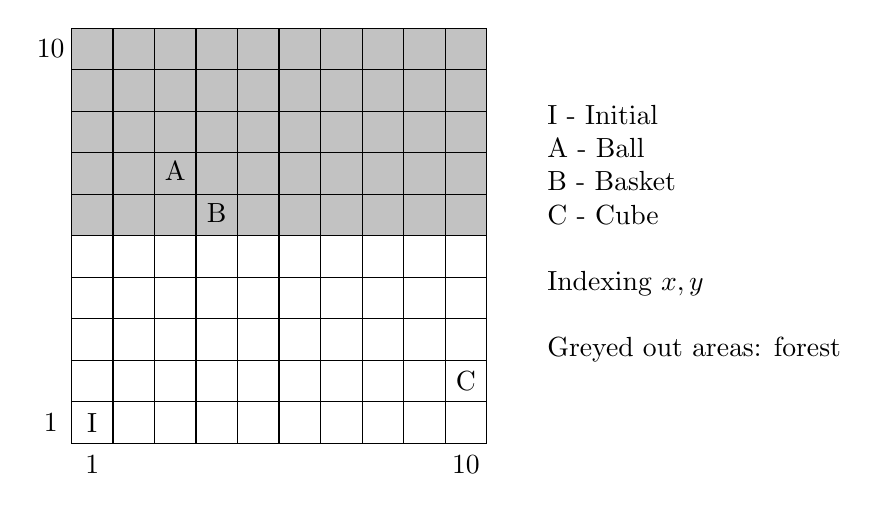
\begin{tikzpicture}[x=0.75pt,y=0.75pt,yscale=-1,xscale=1]
%uncomment if require: \path (0,300); %set diagram left start at 0, and has height of 300

%Shape: Rectangle [id:dp6023317598725679] 
\draw   (160,31) -- (360,31) -- (360,231) -- (160,231) -- cycle ;
%Straight Lines [id:da9595625049929823] 
\draw    (160,51) -- (360,51) ;


%Straight Lines [id:da6847461237580919] 
\draw    (160,71) -- (360,71) ;


%Straight Lines [id:da44024750155121506] 
\draw    (160,91) -- (360,91) ;


%Straight Lines [id:da3881985097326992] 
\draw    (160,211) -- (360,211) ;


%Straight Lines [id:da020750397952615574] 
\draw    (160,111) -- (360,111) ;


%Straight Lines [id:da8540473991045276] 
\draw    (160,131) -- (360,131) ;


%Straight Lines [id:da8795653938952204] 
\draw    (160,151) -- (360,151) ;


%Straight Lines [id:da47867211856391] 
\draw    (160,171) -- (360,171) ;


%Straight Lines [id:da4071178674021898] 
\draw    (160,191) -- (360,191) ;


%Straight Lines [id:da3887731371040415] 
\draw    (180,31) -- (180,231) ;


%Straight Lines [id:da3783849679374176] 
\draw    (200,31) -- (200,231) ;


%Straight Lines [id:da8329815434638699] 
\draw    (220,31) -- (220,231) ;


%Straight Lines [id:da0188961706436912] 
\draw    (240,31) -- (240,231) ;


%Straight Lines [id:da6186048490507579] 
\draw    (260,31) -- (260,231) ;


%Straight Lines [id:da831091260204057] 
\draw    (280,31) -- (280,231) ;


%Straight Lines [id:da5230442661539718] 
\draw    (300,31) -- (300,231) ;


%Straight Lines [id:da6547795584240006] 
\draw    (320,31) -- (320,231) ;


%Straight Lines [id:da6058533775992443] 
\draw    (340,31) -- (340,231) ;


%Shape: Rectangle [id:dp0661789343964958] 
\draw  [fill={rgb, 255:red, 0; green, 0; blue, 0 }  ,fill opacity=0.24 ] (160,31) -- (360,31) -- (360,131) -- (160,131) -- cycle ;

% Text Node
\draw (170,241) node  [align=left] {1};
% Text Node
\draw (150,221) node  [align=left] {1};
% Text Node
\draw (350,241) node  [align=left] {10};
% Text Node
\draw (150,41) node  [align=left] {10};
% Text Node
\draw (210,100) node  [align=left] {A};
% Text Node
\draw (230,120) node  [align=left] {B};
% Text Node
\draw (350,201) node  [align=left] {};
% Text Node
\draw (170,221) node  [align=left] {I};
% Text Node
\draw (350,201) node  [align=left] {C};
% Text Node
\draw (460,130) node  [align=left] {I - Initial\\A - Ball\\B - Basket\\C - Cube\\\\Indexing $\displaystyle x,y$\\\\Greyed out areas: forest};

\end{tikzpicture}



    \caption{Illustration of the modified robot world.}
    \label{fig:robotforest}
\end{figure}
\paragraph{To recap:} The modified robot world shows that if the robot enters the forest areas using $MoveInCity$, without a flashlight, it will be left unable to leave the forest with $MoveInForest$, and will then reach a dead end. As illustrated in Figure \ref{fig:robotforest}. \\

Suppose that the robot is in the City, then there exist no dead end, since the robot will always have the possibility to grab the flashlight before entering the forest. In other words, there is a finite goal distance even if the robot is at the border to the Forest.  \\

Suppose now that a state $s$ where the robot has just entered the Forest without a flashlight is evaluated. The goal distance is now $\infty$ since the robot cannot leave the Forest without a flashlight. H3 does naively ``save'' the previously visited locations, but if the state $s$ is the root of the search, H3 will not have a location in the City saved. Thus H3 will also yield $\infty$, and we have a recognized dead end. \\

Following the quote from the article as shown in the previous subsection, I also deduce that H3 is completeness preserving, as well as defines the state space $(S^\prime, T^\prime)$ which is Recognized. \\

Since these were the two possible scenarios for dead ends in this domain and I cannot find an unrecognized dead end, I conclude that there is none for H3. 

\begin{itemize}
    \item \textit{Does there exist a reachable recognized end for H3?} \\
    Yes. 
    \item \textit{Does there exist a reachable unrecognized end for H3?} \\
    No.
\end{itemize}

\subsection{}

Suppose that we are in a domain as described in Section 4.3. Introduce another heuristics, H5, which ignores the $HasFlashlight(Robot)$ precondition in the action  $MoveInForest$. The H5 state space will naturally be called Unrecognized, since the value of $h_5$ will always be finite (while the goal distance is infinite if robot has entered Forest without flashlight), regardless of if the robot has gone into the forest without a flashlight or not. Now, suppose that the robot is at the border  to the Forest, H5 will suggest that the robot enter the Forest because it is faster than going to fetch the flashlight. If the search algorithm then follows H5 and enters the forest, it will be left without a way out, and it will then be impossible to find a goal, ie impossible to find a solution. Even if a state where the robot has entered the forest without a flashlight is evaluated with H5, the search algorithm will keep searching with H5 since there is no recognized end. 


    
\end{document}

